% ============================================================
%  main.tex — Especificación de Requisitos de Software (ERS/SRS)
%  Proyecto: AquaGest — Sistema para la Gestión Inteligente
%            de Camaroneras (Biofina / Camaronera El Guasmo)
%  Elaborado conforme a la norma ISO/IEC/IEEE 29148:2018
% ============================================================
\documentclass[12pt,a4paper]{article}
\usepackage[utf8]{inputenc}
\usepackage[T1]{fontenc}
\usepackage{cite}
\usepackage{float}
\usepackage{graphicx}
\usepackage{amsmath,amssymb}
\usepackage{url}
\usepackage{longtable}
\usepackage{hyperref}
\usepackage[table]{xcolor}
\usepackage{array}
\usepackage{enumitem}
\hypersetup{colorlinks=true,linkcolor=blue,citecolor=blue,urlcolor=blue}
\usepackage[left=2.5cm,right=2.5cm,top=2.5cm,bottom=2.5cm]{geometry}
\renewcommand{\arraystretch}{1.25}
\renewcommand{\contentsname}{Índice General}
\renewcommand{\figurename}{Figura}
\renewcommand{\tablename}{Tabla}

\begin{document}

\begin{titlepage}
    \centering

    {\Large\textbf{UNIVERSIDAD TÉCNICA ESTATAL DE QUEVEDO}}\\[0.6cm]

    
\includegraphics[width=4cm]{logo.png}\\[0.6cm]

    {\large\textbf{INGENIERÍA DE SOFTWARE}}\\[1cm]

    \textbf{Asignatura:}\\[0.2cm]
    Ingeniería de Requerimientos\\[0.6cm]

    \textbf{Tema:}\\[0.2cm]
    Construcción de la Especificación de Requisitos de Software (ERS/SRS) según la norma ISO/IEC/IEEE 29148\\[0.8cm]

    \textbf{Repositorio GitHub:}\\[0.2cm]
    \url{https://github.com/cperezr3/IR-PFC-GA.git}\\[1cm]

    \textbf{Integrantes:}\\[0.3cm]
    Calle Delgado Kamila Annabella\\
    Macías Herrera Josthyn Esteban\\
    Pérez Ruiz Carlos Andrés\\[0.8cm]

    \textbf{Curso:}\\[0.2cm]
    4to Software ``A''\\[0.6cm]

    \textbf{Docente:}\\[0.2cm]
    Ing. Gleiston Cicerón Guerrero Ulloa\\[0.6cm]

    \textbf{Fecha:}\\[0.2cm]
    08 de Julio de 2026

    \vfill

\end{titlepage}
% ============================================================
\section{Introducción}
% ============================================================

\subsection{Propósito}

El presente documento tiene como propósito especificar de forma clara, completa y verificable los requisitos de software del sistema AquaGest, desarrollado para apoyar la gestión operativa y productiva de la camaronera de la Compañía Biofina, ubicada en el sector El Guasmo. La especificación organiza y documenta los requisitos obtenidos durante el proceso de levantamiento, análisis y validación, siguiendo la estructura propuesta por la norma ISO/IEC/IEEE 29148:2018 para la elaboración de Especificaciones de Requisitos de Software (SRS) \cite{ISO29148:2018}.

Este documento está dirigido al equipo de desarrollo, al docente responsable del proyecto y a los representantes de la Compañía Biofina, con el propósito de establecer un entendimiento común sobre las funcionalidades y restricciones que deberá cumplir el sistema. Asimismo, los requisitos aquí definidos consideran los atributos de calidad establecidos por la norma ISO/IEC/IEEE 29148:2018, como claridad, consistencia, verificabilidad y trazabilidad, mientras que los requisitos no funcionales se organizan de acuerdo con el modelo de calidad propuesto por la norma ISO/IEC 25010:2023 \cite{ISO25010:2023}.

\subsection{Alcance del sistema}

AquaGest es un sistema de información de tipo aplicación web responsiva, sin
instalación en dispositivos de campo, orientado a centralizar y automatizar los
procesos operativos de la camaronera Biofina: gestión de estanques, control de
siembras y crecimiento, monitoreo de parámetros del agua, gestión de
alimentación, historial sanitario, gestión de empleados, control de inventario
y proveedores, mantenimiento de equipos, gestión de cosechas, generación de
reportes comparativos y, como funcionalidades diferenciadoras, un módulo de
inteligencia artificial para la predicción del momento óptimo de cosecha y la
detección de anomalías en los parámetros del agua.

El sistema no reemplaza los procesos productivos físicos de la camaronera (por
ejemplo, la operación manual de aireadores o la aplicación de tratamientos
sanitarios), sino que centraliza su registro, monitoreo y análisis para apoyar
la toma de decisiones del personal operativo y gerencial de Biofina. El alcance
del presente documento corresponde a la versión 1.0 del sistema, resultado del
proceso de clasificación MoSCoW y Kano descrito en la Sección~3 de este
documento, en el cual 14 requisitos fueron clasificados como \textit{Must},
7 como \textit{Should} y 4 como \textit{Could} \cite{Kravchenko2022,Pohl2010}.
Ningún requisito elicitado fue descartado del alcance general del proyecto,
aunque algunos --- particularmente los vinculados a inteligencia artificial ---
están planificados para fases posteriores de incorporación progresiva.

\subsection{Definiciones, acrónimos y abreviaturas}

\begin{longtable}{|p{3.2cm}|p{11cm}|}
\caption{Definiciones, acrónimos y abreviaturas} \\
\hline
\textbf{Término} & \textbf{Definición} \\
\hline
\endfirsthead
\endhead
ERS / SRS & Especificación de Requisitos de Software (\textit{Software Requirements Specification}). \\ \hline
RF & Requisito Funcional. \\ \hline
RNF & Requisito No Funcional. \\ \hline
REST & Restricción del sistema. \\ \hline
RC & Requisito Crudo, identificado durante la fase de elicitación antes de su clasificación. \\ \hline
CU & Caso de Uso. \\ \hline
HU & Historia de Usuario (\textit{User Story}). \\ \hline
BDD & \textit{Behavior-Driven Development}; criterios de aceptación en formato \textit{Given-When-Then} \cite{Cohn2004}. \\ \hline
INVEST & Criterio de calidad de historias de usuario: Independiente, Negociable, Valiosa, Estimable, \textit{Small}, Testeable \cite{Cohn2004}. \\ \hline
MoSCoW & Técnica de priorización \textbf{M}ust, \textbf{S}hould, \textbf{C}ould, \textbf{W}on't \cite{Kravchenko2022}. \\ \hline
FCR & \textit{Food Conversion Ratio}; índice de eficiencia alimenticia. \\ \hline
i* 2.0 & Marco de modelado orientado a metas para la ingeniería de requisitos \textit{Goal-Oriented} \cite{Yu1995,Kavakli2002}. \\ \hline
SD & \textit{Strategic Dependency Model} del marco i* 2.0 \cite{Yu1995}. \\ \hline
SR & \textit{Strategic Rationale Model} del marco i* 2.0 \cite{Yu1995}. \\ \hline
RBAC & Control de acceso basado en roles (\textit{Role-Based Access Control}). \\ \hline
LOPDP & Ley Orgánica de Protección de Datos Personales del Ecuador. \\ \hline
IoT & \textit{Internet of Things}; sensores de campo para captura automatizada de parámetros. \\ \hline
Biofina & Compañía propietaria de la camaronera ubicada en el sector El Guasmo, organización caso de estudio del proyecto AquaGest. \\ \hline
\end{longtable}

\subsection{Referencias}

La elaboración de este documento se fundamenta en el marco normativo
internacional de la Ingeniería de Requisitos, integrado por la norma
ISO/IEC/IEEE 29148:2018 para los procesos y productos de requisitos
\cite{ISO29148:2018}, la norma ISO/IEC/IEEE 15288:2023 para el ciclo de vida de
sistemas \cite{ISO15288:2023}, la norma ISO/IEC/IEEE 12207:2017 para el ciclo de
vida del software \cite{ISO12207:2017}, la norma ISO/IEC 25010:2023 para el
modelo de calidad de producto \cite{ISO25010:2023}, la guía SWEBOK v4.0 del IEEE
Computer Society \cite{SWEBOK2024}, el currículo IREB CPRE Foundation Level
v3.1 \cite{IREB2023} y el PMBoK 7.\textsuperscript{a} edición del PMI
\cite{PMI2021}. Asimismo, se emplean los aportes teóricos de Pohl sobre
fundamentos de la Ingeniería de Requisitos \cite{Pohl2010}, de Robertson y
Robertson sobre dominio de interesados y técnicas de elicitación
\cite{Robertson2012}, de Cohn sobre historias de usuario \cite{Cohn2004}, de Yu
y de Kavakli sobre modelado orientado a metas mediante el marco i*
\cite{Yu1995,Kavakli2002}, de Pacheco et al.\ sobre la efectividad comparada de
técnicas de elicitación \cite{Pacheco2018} y de Kravchenko y Shevgunov sobre la
aplicación práctica del método MoSCoW \cite{Kravchenko2022}. La bibliografía
completa se encuentra consolidada en el archivo \texttt{referencias.bib} en
formato BibTeX y citada en estilo IEEE a lo largo de todo el documento.

\subsection{Visión general del documento}

El resto de este documento se organiza de la siguiente manera. La
Sección~2 presenta la descripción general del producto: su perspectiva,
funciones, clases de usuarios, entorno operativo, restricciones y
suposiciones. La Sección~3 contiene los requisitos específicos del sistema:
requisitos funcionales organizados por módulo, requisitos no funcionales
clasificados según ISO/IEC 25010:2023 \cite{ISO25010:2023}, e interfaces
externas. La Sección~4 presenta los modelos del sistema: actores, casos de
uso y modelo de metas i* 2.0. La Sección~5 documenta las reglas de negocio
identificadas. La Sección~6 organiza los requisitos de calidad por atributo. La
Sección~7 presenta la matriz de trazabilidad entre necesidades del cliente y
requisitos. La Sección~8 identifica los riesgos del proyecto. Finalmente, la
Sección~9 contiene los anexos con la evidencia de la elicitación.


% ============================================================
\section{Descripción General}
% ============================================================

\subsection{Perspectiva del producto}

AquaGest es un producto de software independiente, concebido para sustituir los
registros manuales y dispersos que actualmente emplea la Compañía Biofina en la
gestión de su camaronera. No constituye un componente de un sistema mayor ya
existente, sino un sistema nuevo que centraliza la información generada por los
distintos procesos productivos del negocio acuícola \cite{ISO15288:2023}. Su
perspectiva de producto se deriva directamente del análisis de los procesos
organizacionales de Biofina, realizado mediante entrevista semiestructurada,
cuestionario digital y sesión de brainstorming, conforme al proceso de
definición de requisitos de los interesados establecido en la norma
ISO/IEC/IEEE 15288:2023 \cite{ISO15288:2023} y a los criterios de fuentes de
requisitos de la norma ISO/IEC/IEEE 29148:2018 \cite{ISO29148:2018}.

El sistema deberá operar como una aplicación web responsiva, sin necesidad de
instalación en los dispositivos de campo, dado que el hardware utilizado por el
personal operativo de Biofina es heterogéneo y no administrado centralizadamente
(restricción REST-01, Sección~2.5). Su arquitectura deberá contemplar operación
offline con sincronización diferida, en razón de la conectividad intermitente
propia del entorno de campo de una camaronera \cite{Pohl2010}.

\subsection{Funciones del producto}

De forma resumida, y en correspondencia directa con los requisitos funcionales
especificados en la Sección~3.1, AquaGest deberá proveer las siguientes
funciones principales:

\begin{itemize}[nosep]
  \item Registro y administración de estanques (piscinas), incluyendo su
        capacidad máxima de siembra y su estado operativo.
  \item Registro y trazabilidad de siembras y del crecimiento del camarón
        mediante grameos semanales.
  \item Monitoreo de parámetros fisicoquímicos del agua y generación de
        alertas ante valores fuera de rango.
  \item Cálculo y registro de la alimentación suministrada y de la eficiencia
        alimenticia (FCR) por ciclo.
  \item Registro del historial sanitario de cada estanque y alertas por
        mortalidad anormal.
  \item Gestión de empleados y asignación de tareas diarias.
  \item Gestión de inventario de insumos y de proveedores.
  \item Registro de órdenes de mantenimiento preventivo y correctivo de
        equipos.
  \item Registro de cosechas y cálculo del costo de producción.
  \item Generación de reportes comparativos de producción y gráficas de
        evolución histórica.
  \item Predicción del momento óptimo de cosecha y detección de anomalías en
        los parámetros del agua mediante modelos de inteligencia artificial.
\end{itemize}

Esta enumeración corresponde exactamente al conjunto de 18 requisitos
funcionales (RF-01 a RF-18) obtenidos tras el proceso de clasificación y
eliminación de duplicados descrito en la Sección~3.1, que a su vez se deriva de
los 30 requisitos crudos (RC-01 a RC-30) identificados durante la elicitación
\cite{ISO29148:2018,SWEBOK2024}.

\subsection{Clases de usuarios}

Sobre la base de la identificación de interesados realizada durante la
planificación de la elicitación \cite{PMI2021,Robertson2012}, se reconocen las
siguientes clases de usuarios del sistema AquaGest:

\begin{longtable}{|p{3.6cm}|p{10.6cm}|}
\caption{Clases de usuarios del sistema AquaGest} \\
\hline
\textbf{Clase de usuario} & \textbf{Descripción} \\
\hline
\endfirsthead
\endhead
Administrador de Biofina &
Usuario con visión transversal del proceso productivo y autoridad sobre las
decisiones organizacionales. Clasificado como interesado de alto poder y alto
interés según la matriz poder/interés del PMBoK \cite{PMI2021}. Corresponde al
señor Christian Leonel Franco Anchundia, interesado primario de la entrevista de
elicitación. Supervisa reportes, valida sobrecargas y decisiones de cosecha, y
administra el control de acceso por roles. \\
\hline
Técnico Acuícola &
Usuario directo del módulo de monitoreo de parámetros del agua y del historial
sanitario. Su perspectiva es crítica para la especificación de los umbrales de
alerta y los flujos de excepción del sistema \cite{ISO29148:2018}. Responsable
de diagnosticar y tratar incidentes sanitarios y de registrar acciones
correctivas ante alertas del sistema. \\
\hline
Operario de Producción / Campo &
Usuario directo de los módulos de gestión de piscinas, siembras, alimentación y
grameos. Interesado de bajo poder y alto interés \cite{Robertson2012}. Ejecuta el
registro diario de raciones, grameos y mantenimiento en condiciones operativas
de campo, frecuentemente sin conectividad. \\
\hline
Responsable de Inventario / Bodega &
Usuario del módulo de inventario, responsable de registrar entradas, salidas y
proveedores de insumos (balanceado, medicinas, herramientas, repuestos y
combustible). \\
\hline
Responsable de Mantenimiento &
Usuario del módulo de historial de mantenimiento, responsable de registrar
órdenes preventivas y correctivas de equipos (bombas, aireadores, generadores y
vehículos). \\
\hline
Responsable de Cosecha / Calidad y Empacadora &
Usuario del módulo de cosechas, responsable de registrar el peso total, la
talla promedio y el rendimiento por estanque. \\
\hline
Proveedor de Insumos &
Actor externo al sistema, referenciado como fuente de dependencia en el modelo
i* 2.0 (Sección~4.3). No opera directamente el sistema, pero su información de
contacto e historial de compras es gestionado dentro de AquaGest
\cite{Yu1995}. \\
\hline
Equipo de Desarrollo de AquaGest &
Interesado técnico responsable de transformar los requisitos de los
interesados en requisitos del sistema y software, conforme al proceso de
definición de requisitos de la norma ISO/IEC/IEEE 15288:2023
\cite{ISO15288:2023}. \\
\hline
\end{longtable}

\subsection{Entorno operativo}

AquaGest deberá operar como una aplicación web responsiva, accesible mediante
los navegadores Google Chrome y Mozilla Firefox, sin requerir instalación en los
dispositivos de campo del personal operativo (restricción REST-01,
Sección~2.5). El entorno de operación incluye dispositivos móviles y tablets
utilizados por el personal en el área de piscinas, así como estaciones de
trabajo de escritorio empleadas por el personal administrativo. Dado que la
camaronera se ubica en una zona con conectividad a internet intermitente, el
entorno operativo exige que el sistema soporte un modo de funcionamiento
offline con sincronización automática al restablecerse la conexión, según lo
establecido en el requisito no funcional RNF-01 (Sección~3.2)
\cite{Pohl2010,ISO25010:2023}.

El acta de entrevista de elicitación menciona además la posibilidad de
integración con sensores IoT para la captura automatizada de parámetros del
agua, aunque el flujo de excepción documentado en el caso de uso CU-02
(Sección~4.2) contempla explícitamente el ingreso manual como alternativa ante
fallos del sensor. Otras integraciones de hardware de campo mencionadas
únicamente en la sesión de brainstorming (por ejemplo, balanzas digitales para
el registro automático del peso de cosecha) no fueron promovidas a requisitos
funcionales formales y se documentan como pendientes de definir en futuras
iteraciones.

\subsection{Restricciones}

Las restricciones del sistema AquaGest, identificadas durante el proceso de
elicitación y clasificación de requisitos, se agrupan en restricciones
técnicas, organizacionales y regulatorias, conforme a la definición de
restricción de la norma ISO/IEC/IEEE 29148:2018, según la cual una restricción
es una imposición de diseño o implementación que limita el espacio de
soluciones posibles sin constituir, en sí misma, un comportamiento funcional
\cite{ISO29148:2018}.

\begin{longtable}{|p{1.6cm}|p{2.8cm}|p{9.8cm}|}
\caption{Restricciones del sistema AquaGest} \\
\hline
\textbf{ID} & \textbf{Tipo} & \textbf{Descripción} \\
\hline
\endfirsthead
\endhead
REST-01 & Técnica (Arquitectura) &
El sistema debe desarrollarse como una aplicación web responsiva, compatible
con los navegadores Chrome y Firefox, sin requerir instalación en los
dispositivos de campo \cite{ISO29148:2018}. \\
\hline
REST-02 & Organizacional (Negocio) &
El sistema debe integrarse con los procesos existentes de Biofina sin
modificar los flujos de trabajo de campo durante la etapa de implantación,
condición explícitamente planteada por el stakeholder principal
\cite{Robertson2012}. \\
\hline
REST-03 & Regulatoria (Legal) &
El sistema debe cumplir con la Ley Orgánica de Protección de Datos Personales
(LOPDP) del Ecuador en el tratamiento de los datos del personal de Biofina. \\
\hline
\end{longtable}

Todas las restricciones fueron clasificadas con prioridad \textbf{Must} en el
análisis MoSCoW (Sección~3.1), en razón de su carácter obligatorio para la
viabilidad técnica, organizacional o legal del proyecto \cite{Kravchenko2022}.

\subsection{Suposiciones y dependencias}

El análisis del modelo de metas i* 2.0 (Sección~4.3) permitió identificar las
siguientes suposiciones y dependencias externas del sistema AquaGest
\cite{Yu1995,Kavakli2002}:

\begin{itemize}[nosep]
  \item Se asume que el personal operativo de campo dispondrá de un
        dispositivo móvil o tablet compatible con los navegadores soportados
        (REST-01), condición necesaria para el uso del sistema en las
        instalaciones de la camaronera.
  \item Se asume la existencia de conectividad a internet intermitente pero
        recuperable en un plazo razonable, condición sobre la que se
        fundamenta el diseño de la arquitectura offline-first (RNF-01,
        RNF-04).
  \item El sistema depende de la respuesta oportuna del Proveedor de Insumos
        (actor externo) para la reposición efectiva de stock ante las alertas
        generadas por el módulo de inventario (RF-12); esta dependencia no es
        controlable por AquaGest y constituye una limitación de alcance que
        debe comunicarse explícitamente a la administración de Biofina
        \cite{Yu1995}.
  \item Se asume que existirá un volumen suficiente de datos históricos de
        grameos y parámetros del agua (al menos tres ciclos productivos
        completos) para que el módulo de predicción de cosecha basado en
        inteligencia artificial (RF-17) genere resultados confiables, tal
        como se documenta en el criterio de aceptación BDD de la historia de
        usuario HU-05 (Sección~4.2).
  \item Se asume la disponibilidad y el compromiso de participación de los
        interesados identificados (administrador y personal de las ocho áreas
        operativas) para la validación continua de los requisitos durante las
        siguientes iteraciones del proyecto \cite{PMI2021}.
\end{itemize}


% ============================================================
\section{Requisitos Específicos}
% ============================================================

Los requisitos específicos de AquaGest se derivan del proceso de análisis,
clasificación y eliminación de duplicados aplicado sobre los 30 requisitos
crudos (RC-01 a RC-30) elicitados mediante entrevista, cuestionario digital y
brainstorming. Dicho proceso, descrito con detalle en el proyecto original,
redujo el conjunto a 25 requisitos únicos: 18 requisitos funcionales (RF-01 a
RF-18), 4 requisitos no funcionales (RNF-01 a RNF-04) y 3 restricciones
(REST-01 a REST-03), aplicando como criterios de deduplicación el solapamiento
semántico total y el solapamiento parcial entre requisitos crudos del mismo
dominio \cite{ISO29148:2018,SWEBOK2024}. Cada requisito funcional se redacta
siguiendo los atributos de un buen requisito según la norma
ISO/IEC/IEEE 29148:2018: no ambigüedad, completitud, verificabilidad,
consistencia, necesidad y trazabilidad \cite{ISO29148:2018,Pohl2010}.

% ------------------------------------------------------------
\subsection{Requisitos funcionales}
% ------------------------------------------------------------

Los requisitos funcionales se organizan por módulo funcional, en
correspondencia con las áreas identificadas durante la entrevista y el
cuestionario digital \cite{Robertson2012}. La prioridad de cada requisito
corresponde a la clasificación MoSCoW validada con el stakeholder principal
\cite{Kravchenko2022}. Cuando el documento original no especifica el detalle
completo del flujo paso a paso de un requisito (por disponer únicamente del
diagrama de caso de uso correspondiente, sin su especificación textual), se
indica explícitamente mediante la leyenda ``Pendiente de definir en futuras
iteraciones'', en cumplimiento del principio de no invención de contenido.

%--------------------------------------------------------------
\subsubsection{Módulo: Gestión de Estanques}
%--------------------------------------------------------------

\begin{table}[H]
\centering
\caption{RF-01: Registrar y Actualizar Estanques}
\begin{tabular}{|p{3.6cm}|p{10.4cm}|}
\hline
\textbf{Campo} & \textbf{Descripción} \\
\hline
Identificador & RF-01 \\ \hline
Nombre & Registrar y actualizar estanques \\ \hline
Descripción & El sistema debe permitir registrar y actualizar cada estanque
(piscina) con un código único, superficie en hectáreas, capacidad máxima de
siembra y estado operativo (activo, preparación, cosecha, inactivo), unificando
los requisitos crudos RC-01 y RC-04 \cite{ISO29148:2018}. \\ \hline
Prioridad (MoSCoW) & \textbf{Must} --- elemento base de todos los módulos; sin
registro de estanques no opera ninguna otra funcionalidad \cite{Kravchenko2022}. \\ \hline
Actor & Administrador; Operario de Producción (caso de uso CU-04, Sección~4.2) \\ \hline
Precondiciones & El usuario ha iniciado sesión con un rol autorizado
(RNF-02). \\ \hline
Flujo principal & (1) El usuario accede al módulo de gestión de estanques.
(2) Ingresa o actualiza el código único, la superficie, la capacidad máxima y
el estado del estanque. (3) El sistema valida la información y almacena el
registro. Nota: el flujo detallado paso a paso del caso de uso CU-04 no fue
documentado textualmente en el proyecto original (únicamente se dispone del
diagrama de casos de uso); su especificación completa queda \textbf{pendiente
de definir en futuras iteraciones}. \\ \hline
Postcondiciones & El estanque queda registrado o actualizado y disponible para
su referencia en los módulos de siembra, monitoreo y cosecha. \\ \hline
Criterios de aceptación &
\textbf{Given} que estoy autenticado como administrador,
\textbf{When} registro un nuevo estanque con todos los campos obligatorios,
\textbf{Then} el sistema almacena el registro, asigna un código único y
muestra confirmación de éxito.
\textbf{Given} que un estanque ya existe en el sistema,
\textbf{When} actualizo su estado a ``inactivo'',
\textbf{Then} el sistema registra el cambio y lo refleja en todos los módulos
que referencian ese estanque (Historia de Usuario HU-01) \cite{Cohn2004}. \\ \hline
\end{tabular}
\end{table}

\begin{table}[H]
\centering
\caption{RF-02: Calcular Capacidad Máxima y Registrar Sobrecargas}
\begin{tabular}{|p{3.6cm}|p{10.4cm}|}
\hline
\textbf{Campo} & \textbf{Descripción} \\
\hline
Identificador & RF-02 \\ \hline
Nombre & Calcular capacidad máxima de siembra y registrar sobrecargas
justificadas \\ \hline
Descripción & El sistema debe calcular automáticamente la capacidad máxima de
larvas por estanque en función de su superficie, y permitir el registro de una
sobrecarga controlada acompañada de su justificación, unificando los
requisitos crudos RC-02 y RC-03. \\ \hline
Prioridad (MoSCoW) & \textbf{Must} --- vinculado a RF-01; imprescindible para
controlar la carga de siembra desde la versión inicial. \\ \hline
Actor & Operario de Producción; Administrador (validación de sobrecargas,
según el modelo i* 2.0, Sección~4.3) \\ \hline
Precondiciones & El estanque objetivo está previamente registrado (RF-01). \\ \hline
Flujo principal & El sistema calcula la capacidad máxima al momento de
registrar la siembra (RF-03); si la cantidad de larvas ingresada supera dicha
capacidad, el operario puede registrar una sobrecarga siempre que documente su
justificación. Especificación textual completa del flujo:
\textbf{pendiente de definir en futuras iteraciones}. \\ \hline
Postcondiciones & La capacidad calculada queda asociada al estanque; toda
sobrecarga registrada queda documentada junto con su justificación para
auditoría posterior. \\ \hline
Criterios de aceptación & El sistema no debe permitir el registro de una
siembra por encima de la capacidad máxima calculada sin que se documente
explícitamente la justificación de la sobrecarga. \\ \hline
\end{tabular}
\end{table}

%--------------------------------------------------------------
\subsubsection{Módulo: Control de Siembras}
%--------------------------------------------------------------

\begin{longtable}{|p{3.6cm}|p{10.4cm}|}
\caption{RF-03: Registrar Siembra} \\
\hline
\textbf{Campo} & \textbf{Descripción} \\
\hline
\endfirsthead
Identificador & RF-03 \\ \hline
Nombre & Registrar siembra \\ \hline
Descripción & El sistema debe permitir registrar cada siembra con fecha de
inicio, cantidad de larvas, tipo de larva, laboratorio de origen y responsable
(RC-05). \\ \hline
Prioridad (MoSCoW) & \textbf{Must} --- evento de inicio del ciclo productivo;
su ausencia impide trazar cualquier otro proceso. \\ \hline
Actor & Operario de Producción (Actor principal, CU-01); Administrador (actor
secundario) \\ \hline
Precondiciones & (1) El usuario ha iniciado sesión con rol \textit{Operario} o
\textit{Administrador}. (2) El estanque destino está registrado (RF-01).
(3) El estanque tiene estado ``disponible para siembra''. \\ \hline
Flujo principal &
(1) El actor selecciona ``Registrar Siembra'' en el menú de producción.
(2) El sistema muestra el formulario con fecha, cantidad de larvas, tipo de
larva, laboratorio proveedor y responsable.
(3) El actor completa todos los campos.
(4) El sistema valida la información ingresada.
(5) El sistema almacena el registro en la base de datos (localmente si se
encuentra offline, conforme a RNF-01/RNF-04).
(6) El sistema confirma el registro y actualiza el estado del estanque a
``activo''. \\ \hline
Flujos alternativos &
\textbf{FA1}: en el paso~4, si existen campos incompletos, el sistema resalta
los campos faltantes y solicita corrección, retomando el flujo en el paso~4.
\textbf{FA2}: en el paso~1, si el estanque ya posee una siembra activa, el
sistema impide el registro y muestra el mensaje ``El estanque seleccionado
tiene un ciclo productivo en curso'' (regla de negocio RN-01, Sección~5). \\ \hline
Excepciones & \textbf{E1}: error de conectividad con la base de datos --- el
sistema almacena el registro localmente y programa la sincronización
automática (RNF-01, RNF-04). \\ \hline
Postcondiciones & (1) La siembra queda registrada y trazable por identificador
de ciclo. (2) Se genera una entrada en el historial del ciclo productivo del
estanque. (3) El estado del estanque cambia a ``activo''. \\ \hline
Criterios de aceptación &
\textbf{Given} que existe un estanque con estado ``disponible para siembra'',
\textbf{When} ingreso los datos de siembra y confirmo el registro,
\textbf{Then} el sistema crea el nuevo ciclo productivo, actualiza el estado del
estanque a ``activo'' y genera entrada en el historial.
\textbf{Given} que un estanque ya tiene una siembra activa,
\textbf{When} intento registrar una nueva siembra en ese mismo estanque,
\textbf{Then} el sistema impide el registro y muestra el mensaje de error
correspondiente (Historia de Usuario HU-02) \cite{Cohn2004}. \\ \hline
\end{longtable}

\begin{table}[H]
\centering
\caption{RF-04: Registrar Grameos y Mostrar Historial de Crecimiento}
\begin{tabular}{|p{3.6cm}|p{10.4cm}|}
\hline
\textbf{Campo} & \textbf{Descripción} \\
\hline
Identificador & RF-04 \\ \hline
Nombre & Registrar grameos semanales y mostrar historial de crecimiento \\ \hline
Descripción & El sistema debe registrar los grameos semanales por estanque
(peso promedio, fecha y observaciones) y mostrar el historial de crecimiento
del camarón por ciclo productivo, unificando los requisitos crudos RC-06 y
RC-07. \\ \hline
Prioridad (MoSCoW) & \textbf{Must} --- datos críticos para las decisiones de
alimentación y cosecha, calificados como indispensables por el stakeholder. \\ \hline
Actor & Operario de Producción \\ \hline
Precondiciones & El estanque tiene una siembra activa (RF-03). \\ \hline
Flujo principal & El operario registra el peso promedio semanal, la fecha y
observaciones del grameo; el sistema almacena el dato y actualiza el gráfico de
historial de crecimiento del ciclo. Especificación textual completa del flujo
paso a paso: \textbf{pendiente de definir en futuras iteraciones}. \\ \hline
Postcondiciones & El grameo queda registrado y disponible en el historial de
crecimiento del estanque, insumo directo del módulo de predicción de IA
(RF-17). \\ \hline
Criterios de aceptación & El sistema debe permitir consultar el historial
completo de grameos de un estanque para el ciclo productivo vigente, ordenado
cronológicamente. \\ \hline
\end{tabular}
\end{table}

\begin{table}[H]
\centering
\caption{RF-05: Alerta por Crecimiento Inferior al Esperado}
\begin{tabular}{|p{3.6cm}|p{10.4cm}|}
\hline
\textbf{Campo} & \textbf{Descripción} \\
\hline
Identificador & RF-05 \\ \hline
Nombre & Generar alerta por crecimiento inferior al esperado \\ \hline
Descripción & El sistema debe generar una alerta automática cuando el
crecimiento semanal del camarón sea inferior al esperado para su etapa de
desarrollo (RC-08). \\ \hline
Prioridad (MoSCoW) & \textbf{Should} --- aporta valor operativo, pero el
sistema puede operar con revisión manual en su ausencia. \\ \hline
Actor & Técnico Acuícola; Operario de Producción \\ \hline
Precondiciones & Existe al menos un grameo registrado para el estanque
(RF-04) y un valor de referencia esperado para la etapa del ciclo. \\ \hline
Flujo principal & Al registrarse un nuevo grameo, el sistema compara el
crecimiento observado contra el crecimiento esperado para la etapa; si el valor
es inferior, genera una alerta dirigida al responsable del estanque.
Especificación textual completa del flujo: \textbf{pendiente de definir en
futuras iteraciones}. \\ \hline
Postcondiciones & La alerta queda registrada con su estado (pendiente,
atendida). \\ \hline
Criterios de aceptación & El sistema no debe generar alertas cuando el
crecimiento semanal sea igual o superior al valor esperado para la etapa
correspondiente. \\ \hline
\end{tabular}
\end{table}

%--------------------------------------------------------------
\subsubsection{Módulo: Monitoreo del Agua}
%--------------------------------------------------------------

\begin{longtable}{|p{3.6cm}|p{10.4cm}|}
\caption{RF-06: Registrar Parámetros del Agua y Generar Alertas}
\label{tab:rf06}\\
\hline
\textbf{Campo} & \textbf{Descripción} \\
\hline
\endfirsthead
Identificador & RF-06 \\ \hline
Nombre & Registrar parámetros del agua y generar alertas locales inmediatas \\ \hline
Descripción & El sistema debe permitir registrar mediciones de los parámetros
del agua (pH, oxígeno disuelto, temperatura, salinidad, turbidez y
alcalinidad) y generar alertas locales inmediatas cuando cualquier parámetro
supere o esté por debajo del rango óptimo definido; en modo offline, las
alertas se almacenan localmente y se sincronizan como notificaciones
\textit{push} diferidas al restablecerse la conexión, unificando los
requisitos crudos RC-09 y RC-10 \cite{ISO29148:2018}. Esta redacción es el
resultado de la negociación documentada en el Acta de Negociación
(Sección~9.5) para resolver el conflicto de control identificado entre RF-06 y
RNF-01 \cite{Pohl2010}. \\ \hline
Prioridad (MoSCoW) & \textbf{Must} --- la calidad del agua es el factor de
mayor impacto en la sobrevivencia del camarón. \\ \hline
Actor & Técnico Acuícola (actor principal); Administrador (actor secundario,
receptor de notificaciones \textit{push} diferidas) \\ \hline
Precondiciones & (1) Usuario autenticado con rol \textit{Técnico} o superior
(RNF-02). (2) El estanque objetivo está registrado y en estado activo. \\ \hline
Flujo principal &
(1) El actor selecciona el estanque a monitorear.
(2) El sistema muestra el formulario con los seis parámetros fisicoquímicos.
(3) El actor ingresa los valores medidos.
(4) El sistema valida cada valor contra los rangos óptimos configurados.
(5) El sistema almacena los parámetros con marca de tiempo.
(6) El sistema actualiza el historial de monitoreo del estanque. \\ \hline
Flujos alternativos & \textbf{FA1}: en el paso~4, si algún parámetro está
fuera de rango, el sistema genera una alerta local inmediata en el dispositivo
del técnico; si hay conexión, envía notificación \textit{push} al
administrador; si no hay conexión, almacena la alerta para sincronización
diferida. \textbf{FA2}: en el paso~3, el técnico puede corregir valores mal
digitados antes de guardar, retomando el flujo en el paso~4. \\ \hline
Excepciones & \textbf{E1}: fallo del sensor IoT --- el sistema permite el
ingreso manual de valores y registra la fuente como ``manual'' para
trazabilidad. \\ \hline
Postcondiciones & (1) Los parámetros quedan almacenados con marca de tiempo y
fuente. (2) Se actualiza el historial de monitoreo. (3) Si se generó una
alerta, queda registrada con estado pendiente o enviada. \\ \hline
Criterios de aceptación &
\textbf{Given} que selecciono un estanque activo,
\textbf{When} ingreso los seis parámetros fisicoquímicos dentro de rangos
normales,
\textbf{Then} el sistema guarda la medición con marca de tiempo y actualiza el
historial sin generar alerta.
\textbf{Given} que ingreso un valor de pH fuera del rango óptimo,
\textbf{When} el sistema valida los valores,
\textbf{Then} el sistema genera una alerta local inmediata y la almacena para
sincronización \textit{push} si no hay conexión (Historia de Usuario HU-03)
\cite{Cohn2004}. \\ \hline
\end{longtable}

\begin{table}[H]
\centering
\caption{RF-07: Registrar Acción Correctiva}
\begin{tabular}{|p{3.6cm}|p{10.4cm}|}
\hline
\textbf{Campo} & \textbf{Descripción} \\
\hline
Identificador & RF-07 \\ \hline
Nombre & Registrar acción correctiva ante parámetro fuera de rango \\ \hline
Descripción & El sistema debe registrar la acción correctiva tomada ante un
parámetro del agua fuera de rango, indicando el responsable de ejecutarla y la
fecha (RC-11). \\ \hline
Prioridad (MoSCoW) & \textbf{Should} --- necesario para la trazabilidad de
respuestas operativas; no bloquea la operación inicial. \\ \hline
Actor & Técnico Acuícola \\ \hline
Precondiciones & Existe una alerta generada por un parámetro fuera de rango
(RF-06). \\ \hline
Flujo principal & El técnico registra la acción correctiva ejecutada,
asociándola a la alerta correspondiente, con fecha y responsable.
Especificación textual completa del flujo: \textbf{pendiente de definir en
futuras iteraciones}. \\ \hline
Postcondiciones & La acción correctiva queda registrada y vinculada a la
alerta que la originó, cerrando su ciclo de atención. \\ \hline
Criterios de aceptación & Toda alerta atendida debe contar con un registro de
acción correctiva asociado, con responsable y fecha. \\ \hline
\end{tabular}
\end{table}

%--------------------------------------------------------------
\subsubsection{Módulo: Alimentación}
%--------------------------------------------------------------

\begin{table}[H]
\centering
\caption{RF-08: Calcular y Registrar Alimentación Diaria}
\begin{tabular}{|p{3.6cm}|p{10.4cm}|}
\hline
\textbf{Campo} & \textbf{Descripción} \\
\hline
Identificador & RF-08 \\ \hline
Nombre & Calcular ración diaria y registrar alimentación suministrada \\ \hline
Descripción & El sistema debe calcular la ración diaria de alimento por
estanque en función de la biomasa estimada y la etapa de crecimiento, y
registrar diariamente el tipo de alimento, la cantidad suministrada, el
horario, el estanque y el operario responsable, unificando los requisitos
crudos RC-12 y RC-13. \\ \hline
Prioridad (MoSCoW) & \textbf{Must} --- el alimento representa el mayor costo
operativo; su gestión es obligatoria desde el inicio. \\ \hline
Actor & Operario de Producción / Campo \\ \hline
Precondiciones & El estanque tiene una siembra activa (RF-03) y datos de
grameo recientes (RF-04) que permiten estimar la biomasa. \\ \hline
Flujo principal & El sistema calcula la ración recomendada según la biomasa
estimada y la etapa de crecimiento; el operario confirma o ajusta la cantidad
suministrada y el sistema registra la transacción diaria. Especificación
textual completa del flujo: \textbf{pendiente de definir en futuras
iteraciones}. \\ \hline
Postcondiciones & Queda registrada la alimentación diaria por estanque,
insumo directo del cálculo de eficiencia alimenticia (RF-09). \\ \hline
Criterios de aceptación & El sistema debe registrar cada suministro de
alimento con tipo, cantidad, horario, estanque y operario responsable. \\ \hline
\end{tabular}
\end{table}

\begin{table}[H]
\centering
\caption{RF-09: Generar Informe de Eficiencia Alimenticia (FCR)}
\begin{tabular}{|p{3.6cm}|p{10.4cm}|}
\hline
\textbf{Campo} & \textbf{Descripción} \\
\hline
Identificador & RF-09 \\ \hline
Nombre & Generar informe de eficiencia alimenticia (FCR) \\ \hline
Descripción & El sistema debe generar un informe de eficiencia alimenticia
(\textit{Food Conversion Ratio}) por ciclo productivo (RC-14). \\ \hline
Prioridad (MoSCoW) & \textbf{Should} --- complemento analítico de RF-08;
importante pero no bloqueante para la operación básica. \\ \hline
Actor & Administrador \\ \hline
Precondiciones & Existen registros de alimentación (RF-08) y de cosecha o
biomasa del ciclo. \\ \hline
Flujo principal & El sistema calcula el FCR a partir del alimento suministrado
acumulado y la ganancia de biomasa del ciclo, y presenta el resultado en el
informe correspondiente. Especificación textual completa del flujo:
\textbf{pendiente de definir en futuras iteraciones}. \\ \hline
Postcondiciones & El informe de FCR queda disponible para consulta y
comparación entre ciclos (RF-16). \\ \hline
Criterios de aceptación & El informe de FCR debe poder generarse para
cualquier ciclo productivo cerrado que cuente con registros completos de
alimentación. \\ \hline
\end{tabular}
\end{table}


%--------------------------------------------------------------
\subsubsection{Módulo: Historial Sanitario}
%--------------------------------------------------------------

\begin{table}[H]
\centering
\caption{RF-10: Registrar Incidentes Sanitarios y Alertar Mortalidad Anormal}
\begin{tabular}{|p{3.6cm}|p{10.4cm}|}
\hline
\textbf{Campo} & \textbf{Descripción} \\
\hline
Identificador & RF-10 \\ \hline
Nombre & Registrar incidentes sanitarios y alertar por mortalidad anormal \\ \hline
Descripción & El sistema debe permitir registrar incidentes sanitarios con
fecha, síntomas observados, diagnóstico y tratamiento aplicado, y alertar al
técnico acuícola cuando se registre una mortalidad anormal en un estanque,
unificando los requisitos crudos RC-15 y RC-16. \\ \hline
Prioridad (MoSCoW) & \textbf{Must} --- la detección temprana de enfermedades
puede evitar pérdidas totales de un estanque. \\ \hline
Actor & Técnico Acuícola (caso de uso CU-08, Sección~4.2) \\ \hline
Precondiciones & El estanque objeto del incidente está registrado y en estado
activo. \\ \hline
Flujo principal & El técnico registra el incidente sanitario con fecha,
síntomas, diagnóstico y tratamiento; si el nivel de mortalidad reportado
excede el umbral configurado, el sistema genera una alerta dirigida al
técnico responsable. Especificación textual completa del flujo paso a paso
del caso de uso CU-08: \textbf{pendiente de definir en futuras iteraciones}
(el proyecto original únicamente referencia su diagrama, Figura~8). \\ \hline
Postcondiciones & El incidente sanitario queda registrado en el historial del
estanque; si se generó alerta, queda registrada con su estado. \\ \hline
Criterios de aceptación & Toda mortalidad registrada por encima del umbral
configurado debe generar una alerta automática dirigida al técnico
responsable. \\ \hline
\end{tabular}
\end{table}

%--------------------------------------------------------------
\subsubsection{Módulo: Gestión de Empleados}
%--------------------------------------------------------------

\begin{table}[H]
\centering
\caption{RF-11: Registrar Empleados y Asignar Tareas}
\begin{tabular}{|p{3.6cm}|p{10.4cm}|}
\hline
\textbf{Campo} & \textbf{Descripción} \\
\hline
Identificador & RF-11 \\ \hline
Nombre & Registrar empleados y asignar tareas diarias \\ \hline
Descripción & El sistema debe registrar empleados con nombre, cédula, cargo,
rol en el sistema y fecha de ingreso, y permitir asignarles tareas diarias por
área con registro de su cumplimiento, unificando los requisitos crudos RC-17 y
RC-18. \\ \hline
Prioridad (MoSCoW) & \textbf{Should} --- mejora la gestión operativa, pero
puede controlarse manualmente en la versión inicial. \\ \hline
Actor & Administrador \\ \hline
Precondiciones & El usuario está autenticado con rol \textit{Administrador}
(RNF-02). \\ \hline
Flujo principal & El administrador registra los datos del empleado y su rol en
el sistema, y le asigna tareas diarias por área; el empleado o su supervisor
registra el cumplimiento de la tarea asignada. Especificación textual completa
del flujo: \textbf{pendiente de definir en futuras iteraciones}. \\ \hline
Postcondiciones & El empleado queda registrado con su rol asignado; las
tareas diarias quedan registradas con su estado de cumplimiento. \\ \hline
Criterios de aceptación & Todo empleado registrado debe tener asociado un rol
del sistema válido (administrador, técnico u operario, conforme a RNF-02). \\ \hline
\end{tabular}
\end{table}

%--------------------------------------------------------------
\subsubsection{Módulo: Inventario / Bodega}
%--------------------------------------------------------------

\begin{table}[H]
\centering
\caption{RF-12: Gestionar Inventario de Insumos y Alertar Stock Mínimo}
\begin{tabular}{|p{3.6cm}|p{10.4cm}|}
\hline
\textbf{Campo} & \textbf{Descripción} \\
\hline
Identificador & RF-12 \\ \hline
Nombre & Gestionar inventario de insumos y alertar por stock bajo el mínimo \\ \hline
Descripción & El sistema debe gestionar el inventario de insumos (balanceado,
medicinas, herramientas, repuestos y combustible), registrando entradas,
salidas y stock actual, y generar una alerta cuando el stock de un insumo
crítico sea inferior al nivel mínimo configurado, unificando los requisitos
crudos RC-19 y RC-20. \\ \hline
Prioridad (MoSCoW) & \textbf{Must} --- los cortes de insumos detienen la
producción; funcionalidad crítica desde el inicio. \\ \hline
Actor & Responsable de Inventario / Bodega (caso de uso CU-05, Sección~4.2);
Administrador \\ \hline
Precondiciones & El insumo objeto de la transacción está registrado en el
inventario. \\ \hline
Flujo principal &
(1) El bodeguero registra una entrada o salida de inventario.
(2) El sistema actualiza el stock actual del insumo.
(3) El sistema evalúa si el nuevo stock es inferior al nivel mínimo
configurado. \\ \hline
Flujo alternativo & Si el stock resultante es inferior al mínimo configurado,
el sistema genera automáticamente una alerta de reposición visible para el
administrador. \\ \hline
Postcondiciones & La transacción de inventario queda registrada con fecha,
cantidad y responsable; si corresponde, la alerta de stock mínimo queda
registrada. \\ \hline
Criterios de aceptación &
\textbf{Given} que existe stock registrado de un insumo,
\textbf{When} registro una salida de inventario,
\textbf{Then} el sistema actualiza el stock y registra la transacción con
fecha, cantidad y responsable.
\textbf{Given} que el stock de un insumo crítico cae por debajo del nivel
mínimo configurado,
\textbf{When} el sistema procesa la salida de inventario,
\textbf{Then} el sistema genera automáticamente una alerta de reposición
visible para el administrador (Historia de Usuario HU-04) \cite{Cohn2004}. \\ \hline
\end{tabular}
\end{table}

\begin{table}[H]
\centering
\caption{RF-13: Registrar Proveedores e Historial de Compras}
\begin{tabular}{|p{3.6cm}|p{10.4cm}|}
\hline
\textbf{Campo} & \textbf{Descripción} \\
\hline
Identificador & RF-13 \\ \hline
Nombre & Registrar proveedores de insumos e historial de compras \\ \hline
Descripción & El sistema debe registrar los proveedores de insumos con su
información de contacto y mantener un historial de compras por proveedor
(RC-29, derivado de la idea de brainstorming B14). \\ \hline
Prioridad (MoSCoW) & \textbf{Could} --- agrega valor a la gestión de compras,
pero no es crítico para la versión inicial. \\ \hline
Actor & Responsable de Inventario / Bodega; Proveedor de Insumos (actor
externo, modelo i* 2.0, Sección~4.3) \\ \hline
Precondiciones & El usuario está autenticado con un rol autorizado para
gestionar el módulo de inventario. \\ \hline
Flujo principal & El bodeguero registra los datos de contacto del proveedor;
cada compra realizada a dicho proveedor queda asociada a su historial.
Especificación textual completa del flujo: \textbf{pendiente de definir en
futuras iteraciones}. \\ \hline
Postcondiciones & El proveedor queda registrado con su información de
contacto; el historial de compras queda disponible para consulta. \\ \hline
Criterios de aceptación & El sistema debe permitir consultar el historial
completo de compras asociado a un proveedor específico. \\ \hline
\end{tabular}
\end{table}

%--------------------------------------------------------------
\subsubsection{Módulo: Mantenimiento}
%--------------------------------------------------------------

\begin{table}[H]
\centering
\caption{RF-14: Registrar Órdenes de Mantenimiento}
\begin{tabular}{|p{3.6cm}|p{10.4cm}|}
\hline
\textbf{Campo} & \textbf{Descripción} \\
\hline
Identificador & RF-14 \\ \hline
Nombre & Registrar órdenes de mantenimiento de equipos \\ \hline
Descripción & El sistema debe registrar las órdenes de mantenimiento
(preventivo y correctivo) de los equipos productivos: bombas, aireadores,
generadores y vehículos (RC-21). \\ \hline
Prioridad (MoSCoW) & \textbf{Should} --- el mantenimiento preventivo reduce
paros; puede gestionarse externamente en la versión 1. \\ \hline
Actor & Responsable de Mantenimiento \\ \hline
Precondiciones & El equipo objeto de la orden está identificado en el sistema. \\ \hline
Flujo principal & El responsable de mantenimiento registra el tipo de orden
(preventiva o correctiva), el equipo afectado y la descripción del trabajo
realizado. Especificación textual completa del flujo: \textbf{pendiente de
definir en futuras iteraciones}. \\ \hline
Postcondiciones & La orden de mantenimiento queda registrada en el historial
del equipo correspondiente. \\ \hline
Criterios de aceptación & El sistema debe permitir consultar el historial de
órdenes de mantenimiento de un equipo específico, clasificadas por tipo
(preventivo o correctivo). \\ \hline
\end{tabular}
\end{table}

%--------------------------------------------------------------
\subsubsection{Módulo: Gestión de Cosechas}
%--------------------------------------------------------------

\begin{table}[H]
\centering
\caption{RF-15: Registrar Cosecha y Calcular Costo de Producción}
\begin{tabular}{|p{3.6cm}|p{10.4cm}|}
\hline
\textbf{Campo} & \textbf{Descripción} \\
\hline
Identificador & RF-15 \\ \hline
Nombre & Registrar cosecha y calcular costo de producción \\ \hline
Descripción & El sistema debe registrar cada cosecha con fecha, estanque,
peso total, talla promedio y rendimiento (libras/hectárea), y calcular el
costo de producción por cosecha incluyendo alimento, insumos y mano de obra,
unificando los requisitos crudos RC-22 y RC-23. \\ \hline
Prioridad (MoSCoW) & \textbf{Must} --- el cierre del ciclo y el control de
costos son obligatorios para la viabilidad económica. \\ \hline
Actor & Operario de Producción; Administrador (caso de uso CU-06,
Sección~4.2) \\ \hline
Precondiciones & El estanque tiene una siembra activa próxima a su cierre de
ciclo (RF-03). \\ \hline
Flujo principal & El operario registra los datos de la cosecha (fecha, peso
total, talla promedio); el sistema calcula el rendimiento por hectárea y el
costo total de producción a partir de los registros de alimentación (RF-08),
insumos (RF-12) y mano de obra. Especificación textual completa del flujo del
caso de uso CU-06: \textbf{pendiente de definir en futuras iteraciones}. \\ \hline
Postcondiciones & La cosecha queda registrada; el estado del estanque cambia a
``cosecha'' o ``disponible para siembra''; el costo de producción queda
disponible para los reportes comparativos (RF-16). \\ \hline
Criterios de aceptación & El sistema debe calcular el rendimiento
(libras/hectárea) y el costo total de producción de cada cosecha registrada,
de forma consistente con los registros de alimentación e insumos del ciclo. \\ \hline
\end{tabular}
\end{table}

%--------------------------------------------------------------
\subsubsection{Módulo: Reportes}
%--------------------------------------------------------------

\begin{table}[H]
\centering
\caption{RF-16: Generar Reportes Comparativos y Gráficas de Evolución}
\begin{tabular}{|p{3.6cm}|p{10.4cm}|}
\hline
\textbf{Campo} & \textbf{Descripción} \\
\hline
Identificador & RF-16 \\ \hline
Nombre & Generar reportes comparativos de producción y gráficas de evolución
histórica \\ \hline
Descripción & El sistema debe generar reportes comparativos de producción
entre ciclos productivos y gráficas de evolución histórica de los parámetros
del agua por estanque y período de tiempo seleccionable, unificando los
requisitos crudos RC-24 y RC-30. \\ \hline
Prioridad (MoSCoW) & \textbf{Should} --- apoyo a la toma de decisiones
directivas; no impide la operación básica inicial. \\ \hline
Actor & Administrador (caso de uso CU-03) \\ \hline
Precondiciones & (1) El usuario está autenticado con rol \textit{Administrador}.
(2) Existen registros de producción para el período seleccionado. \\ \hline
Flujo principal &
(1) El actor accede al menú ``Reportes''.
(2) El actor selecciona el período de análisis.
(3) El actor selecciona el estanque o ciclo productivo a reportar (o
``todos'').
(4) El actor solicita la generación del reporte.
(5) El sistema procesa y consolida la información de producción, alimentación,
cosechas y parámetros del agua.
(6) El sistema genera el reporte en formato PDF.
(7) El actor descarga o visualiza el documento. \\ \hline
Flujos alternativos & \textbf{FA1}: en el paso~7, si el actor elige exportar a
Excel, el sistema genera el archivo \texttt{.xlsx} con los mismos datos
tabulados. \textbf{FA2}: en el paso~3, el actor puede aplicar filtros
adicionales (área funcional, parámetro específico, empleado), retomando el
flujo en el paso~4. \\ \hline
Excepciones & \textbf{E1}: no existen datos para el período seleccionado ---
el sistema muestra el mensaje ``Sin registros para el período indicado'' y no
genera el reporte. \\ \hline
Postcondiciones & (1) El reporte queda disponible para descarga durante la
sesión activa. (2) Queda registro de auditoría del reporte generado (usuario,
fecha, parámetros de filtro). \\ \hline
Criterios de aceptación & El sistema debe generar el reporte solicitado en
formato PDF o Excel únicamente cuando existan registros de producción para el
período y el filtro seleccionados; en caso contrario, debe informar la
ausencia de datos sin generar un documento vacío. \\ \hline
\end{tabular}
\end{table}

%--------------------------------------------------------------
\subsubsection{Módulo: Inteligencia Artificial}
%--------------------------------------------------------------

\begin{table}[H]
\centering
\caption{RF-17: Módulo de IA para Predicción del Momento Óptimo de Cosecha}
\begin{tabular}{|p{3.6cm}|p{10.4cm}|}
\hline
\textbf{Campo} & \textbf{Descripción} \\
\hline
Identificador & RF-17 \\ \hline
Nombre & Predecir el momento óptimo de cosecha mediante inteligencia
artificial \\ \hline
Descripción & El sistema debe incorporar un módulo de inteligencia artificial
que prediga el momento óptimo de cosecha con base en el historial de grameos
(RF-04) y los parámetros del agua (RF-06) (RC-25). \\ \hline
Prioridad (MoSCoW) & \textbf{Could} --- requiere datos históricos acumulados;
aplica en versiones posteriores. Clasificado como requisito
\textit{Atractivo} en el modelo de Kano \cite{Pohl2010}. \\ \hline
Actor & Administrador (caso de uso CU-07); Módulo IA (actor secundario de
soporte) \\ \hline
Precondiciones & Existen al menos tres ciclos productivos históricos con
grameos semanales completos. \\ \hline
Flujo principal & El administrador ejecuta el módulo de predicción para un
estanque activo; el sistema procesa el historial de grameos y parámetros del
agua disponibles y genera la fecha de cosecha óptima con un intervalo de
confianza. \\ \hline
Excepciones & Si los datos históricos son insuficientes (menos de tres
ciclos), el sistema muestra el aviso ``Datos históricos insuficientes para
generar predicción confiable'' y no ejecuta el modelo. \\ \hline
Postcondiciones & La predicción generada queda disponible en el panel del
administrador junto con su intervalo de confianza. \\ \hline
Criterios de aceptación &
\textbf{Given} que existen al menos tres ciclos productivos históricos con
grameos semanales completos,
\textbf{When} ejecuto el módulo de predicción IA para un estanque activo,
\textbf{Then} el sistema genera la fecha de cosecha óptima con un intervalo de
confianza y la muestra en el panel del administrador.
\textbf{Given} que los datos históricos son insuficientes,
\textbf{When} intento ejecutar el módulo de predicción IA,
\textbf{Then} el sistema muestra el aviso correspondiente y no ejecuta el
modelo (Historia de Usuario HU-05) \cite{Cohn2004}. \\ \hline
\end{tabular}
\end{table}

\begin{table}[H]
\centering
\caption{RF-18: Detección de Anomalías en Parámetros del Agua}
\begin{tabular}{|p{3.6cm}|p{10.4cm}|}
\hline
\textbf{Campo} & \textbf{Descripción} \\
\hline
Identificador & RF-18 \\ \hline
Nombre & Detectar anomalías en parámetros del agua mediante aprendizaje
automático \\ \hline
Descripción & El sistema debe detectar automáticamente anomalías en los
parámetros del agua mediante un algoritmo de aprendizaje automático y
notificar al técnico responsable (RC-27, derivado de la idea de brainstorming
B12). \\ \hline
Prioridad (MoSCoW) & \textbf{Could} --- complemento avanzado de RF-06; requiere
volumen de datos suficiente. Planificado para fase~2. Clasificado como
requisito \textit{Atractivo} en el modelo de Kano \cite{Pohl2010}. \\ \hline
Actor & Módulo IA (actor secundario); Técnico Acuícola (receptor de la
notificación) \\ \hline
Precondiciones & Existe un volumen histórico suficiente de mediciones de
parámetros del agua (RF-06) para el entrenamiento o la ejecución del modelo. \\ \hline
Flujo principal & El módulo de IA analiza continuamente las mediciones
registradas y, al detectar un patrón anómalo distinto de una simple superación
de rango, notifica al técnico acuícola responsable. Especificación textual
completa del flujo: \textbf{pendiente de definir en futuras iteraciones}. \\ \hline
Postcondiciones & La anomalía detectada queda registrada junto con la
notificación generada al técnico responsable. \\ \hline
Criterios de aceptación & El sistema debe distinguir entre una alerta de rango
simple (RF-06) y una anomalía detectada por el modelo de aprendizaje
automático, registrando ambas de forma diferenciada. \\ \hline
\end{tabular}
\end{table}


% ------------------------------------------------------------
\subsection{Requisitos no funcionales}
% ------------------------------------------------------------

Los requisitos no funcionales se clasifican utilizando el vocabulario de
características de calidad de la norma ISO/IEC 25010:2023
\cite{ISO25010:2023}. El documento original identificó cuatro requisitos no
funcionales principales (RNF-01 a RNF-04) y tres requisitos de seguridad
adicionales derivados del análisis del \textit{misuse scenario} MS-01
(Sección~6). Para las categorías no cubiertas explícitamente por el documento
original se indica expresamente su ausencia de información.

\begin{longtable}{|p{2.6cm}|p{1.4cm}|p{9.8cm}|}
\caption{Requisitos no funcionales del sistema AquaGest} \\
\hline
\textbf{Categoría} & \textbf{ID} & \textbf{Descripción} \\
\hline
\endfirsthead
\hline
\textbf{Categoría} & \textbf{ID} & \textbf{Descripción} \\
\hline
\endhead

Disponibilidad & RNF-01 &
El sistema debe mantener una disponibilidad igual o superior al 99\,\% mensual
y operar en modo offline con sincronización automática, soportando al menos
4 horas de operación autónoma sin conectividad (RC-26). \textbf{Prioridad
MoSCoW: Must.} Redacción actualizada tras la negociación de requisitos que
resolvió el conflicto de control con RF-06 (Sección~9.5) \cite{Pohl2010}. \\
\hline

Seguridad & RNF-02 &
El sistema debe implementar autenticación multifactor y control de acceso
basado en roles (administrador, técnico, operario) (RC-28). \textbf{Prioridad
MoSCoW: Must.} \\
\hline

Seguridad & RNF-SEG-01 &
El sistema debe bloquear temporalmente una cuenta durante 15 minutos después
de tres intentos fallidos consecutivos de autenticación, y notificar al
administrador del evento. Requisito derivado del análisis del \textit{misuse
scenario} MS-01 (Sección~6) \cite{Pohl2010,SWEBOK2024}. \\
\hline

Seguridad & RNF-SEG-02 &
El sistema debe almacenar todas las contraseñas mediante algoritmos de hash
seguro con sal (\textit{bcrypt} o equivalente aprobado por el NIST), sin
almacenar contraseñas en texto plano ni en formatos reversibles. \\
\hline

Seguridad & RNF-SEG-03 &
El sistema debe implementar control de acceso basado en roles (RBAC) que
restrinja cada punto de acceso y funcionalidad según el rol asignado al
usuario autenticado, rechazando solicitudes de recursos fuera del rol con
código de respuesta HTTP 403. \\
\hline

Rendimiento & RNF-03 &
El sistema debe responder a consultas históricas en menos de 3 segundos con
hasta 15 usuarios concurrentes (RC-09, RC-24). \textbf{Prioridad MoSCoW:
Should.} \\
\hline

Confiabilidad & RNF-04 &
El sistema no debe perder datos ante fallos de conectividad o energía;
las transacciones deben persistirse localmente y sincronizarse sin pérdida al
restablecerse la conexión (RC-26). \textbf{Prioridad MoSCoW: Must.} \\
\hline

Usabilidad & --- &
El modelo de metas i* 2.0 (Sección~4.3) identifica la usabilidad del sistema en
condiciones de campo (interfaz simple e intuitiva) como una vulnerabilidad
(\textit{softgoal}) crítica del Operario de Campo, dado su menor nivel de
capacitación tecnológica. El documento original no especifica métricas
cuantitativas de usabilidad (por ejemplo, tiempo de aprendizaje o tasa de
error); su definición precisa queda \textbf{pendiente de definir en futuras
iteraciones}. \\
\hline

Escalabilidad & --- &
El documento original no contiene información suficiente sobre requisitos de
escalabilidad (por ejemplo, crecimiento proyectado del número de estanques,
usuarios concurrentes más allá de los 15 indicados en RNF-03, o volumen de
datos históricos). \textbf{Pendiente de definir en futuras iteraciones.} \\
\hline

Mantenibilidad & --- &
El modelo SR del actor Sistema AquaGest (Sección~4.3) identifica la
mantenibilidad del código ante cambios en los procesos de Biofina como una
vulnerabilidad (\textit{softgoal}) del sistema, sin que el documento original
defina métricas o criterios cuantitativos de mantenibilidad conforme a
ISO/IEC 25010:2023 \cite{ISO25010:2023}. Su especificación detallada queda
\textbf{pendiente de definir en futuras iteraciones}. \\
\hline

Compatibilidad & --- &
Cubierta parcialmente por la restricción técnica REST-01 (Sección~2.5):
compatibilidad con los navegadores Chrome y Firefox. No se dispone de
información adicional sobre compatibilidad con otros sistemas o formatos de
intercambio de datos más allá de la exportación a PDF y Excel (RF-16).
\textbf{Pendiente de definir en futuras iteraciones} para aspectos adicionales
de compatibilidad. \\
\hline

Portabilidad & --- &
El documento original no contiene información específica sobre requisitos de
portabilidad del sistema entre distintos entornos de despliegue (por ejemplo,
contenedores, proveedores de nube o migración de base de datos).
\textbf{Pendiente de definir en futuras iteraciones.} \\
\hline
\end{longtable}

% ------------------------------------------------------------
\subsection{Interfaces externas}
% ------------------------------------------------------------

\subsubsection{Interfaces de usuario}

El sistema debe proveerse como una aplicación web responsiva accesible desde
navegadores de escritorio y dispositivos móviles (REST-01), con formularios de
registro accesibles en modo offline para el personal de campo, condición
identificada como \textit{softgoal} crítico del Operario de Campo en el modelo
i* 2.0 (Sección~4.3) \cite{Yu1995}. Durante la sesión de brainstorming se
propusieron, además, un panel de control (\textit{dashboard}) en tiempo real de
los parámetros del agua de cada estanque y un mapa visual de estanques con
codificación por colores según su estado; ambas ideas fueron valoradas con
prioridad alta y media respectivamente por el equipo de desarrollo, aunque no
fueron promovidas formalmente a un requisito funcional único dentro del
conjunto RF-01 a RF-18, por lo que su especificación de interfaz detallada
queda \textbf{pendiente de definir en futuras iteraciones}.

\subsubsection{Interfaces de hardware}

El caso de uso CU-02 (Sección~4.2) contempla la integración con sensores IoT
para la captura automatizada de los parámetros del agua, incluyendo un flujo de
excepción ante fallo del sensor que permite el ingreso manual de valores. La
idea de brainstorming B06 (integración con balanzas digitales para el registro
automático del peso durante la cosecha) fue valorada con prioridad media, pero
no fue incorporada al conjunto de requisitos crudos consolidados (RC-01 a
RC-30) ni, por consiguiente, a los requisitos funcionales RF-01 a RF-18; su
especificación de interfaz de hardware queda \textbf{pendiente de definir en
futuras iteraciones}.

\subsubsection{Interfaces de software}

El sistema debe soportar la exportación de reportes en formato PDF y en
formato Excel (\texttt{.xlsx}) (RF-16). El documento original no especifica
interfaces de integración con sistemas externos de terceros (por ejemplo, un
ERP contable o un sistema de nómina), por lo que estas interfaces quedan
\textbf{pendientes de definir en futuras iteraciones}.

\subsubsection{Interfaces de comunicación}

El sistema debe soportar la sincronización de datos entre el modo offline y el
servidor central al restablecerse la conectividad (RNF-01, RNF-04), así como el
envío de notificaciones \textit{push} diferidas al administrador o supervisor
cuando se genere una alerta en modo offline (RF-06). La idea de brainstorming
B02 (alerta por SMS ante niveles críticos de oxígeno disuelto) fue valorada con
prioridad alta, pero no fue incorporada al conjunto de requisitos crudos
consolidados; su especificación como canal de comunicación adicional queda
\textbf{pendiente de definir en futuras iteraciones}.


% ============================================================
\section{Modelos del Sistema}
% ============================================================

\subsection{Actores del sistema}

El análisis de casos de uso y el modelo de metas i*~2.0 (Sección~4.3)
identifican de forma consistente cinco actores para el sistema AquaGest
\cite{Yu1995,Kavakli2002}: el \textbf{Administrador de Biofina}, el
\textbf{Técnico Acuícola}, el \textbf{Operario de Producción / Campo}, el
\textbf{Sistema AquaGest} en su rol de agente de software (que incluye el
\textbf{Módulo IA} como componente de soporte) y el \textbf{Proveedor de
Insumos} como actor externo. Estos actores corresponden a las clases de
usuarios descritas en la Sección~2.3.

\subsection{Diagrama de casos de uso UML}

El diagrama de casos de uso del sistema AquaGest identifica ocho casos de uso
principales distribuidos entre cuatro actores: Operario de Producción, Técnico
Acuícola, Administrador y Módulo IA (actor secundario de soporte). El límite
del sistema delimita las funcionalidades bajo responsabilidad directa de
AquaGest \cite{ISO29148:2018,SWEBOK2024}.

\begin{table}[H]
\centering
\caption{Resumen de actores y casos de uso del sistema AquaGest}
\begin{tabular}{|p{2.8cm}|p{1.5cm}|p{5.5cm}|p{4.2cm}|}
\hline
\textbf{Actor} & \textbf{ID CU} & \textbf{Nombre del Caso de Uso} & \textbf{Relaciones UML} \\
\hline
Operario de Producción & CU-01 & Registrar Siembra & \textit{include} Validar Estanque \\
\hline
Técnico Acuícola & CU-02 & Registrar Parámetros del Agua & \textit{extend} Generar Alerta \\
\hline
Administrador & CU-03 & Generar Reporte Productivo & \textit{extend} Exportar a Excel \\
\hline
Operario / Administrador & CU-04 & Gestionar Estanques & \textit{include} Verificar Rangos \\
\hline
Bodeguero / Administrador & CU-05 & Gestionar Inventario & \textit{extend} Generar Alerta Stock \\
\hline
Operario / Administrador & CU-06 & Registrar Cosecha & \textit{include} Calcular Costo Producción \\
\hline
Administrador & CU-07 & Consultar Predicciones IA & \textit{include} Módulo IA (actor) \\
\hline
Técnico Acuícola & CU-08 & Registrar Incidentes Sanitarios & \textit{extend} Alertar Mortalidad Anormal \\
\hline
\end{tabular}
\end{table}

\noindent\textbf{Nota:} las relaciones de generalización agrupan a Operario y
Técnico Acuícola bajo el rol genérico \textit{Usuario de Campo}; Administrador
generaliza sobre todos los actores operativos para las funciones de
supervisión y reportes.

\subsection{Especificación de casos de uso}

Se reproducen a continuación los tres casos de uso especificados
textualmente en el proyecto original (CU-01, CU-02 y CU-03), en
correspondencia directa con los requisitos RF-03/RF-04, RF-06/RF-07 y RF-16
respectivamente, y se documentan los diagramas de los cinco casos de uso
restantes (CU-04 a CU-08), para los cuales el proyecto original únicamente
proporciona el diagrama gráfico sin especificación textual de flujo.

\subsubsection{CU-01: Registrar Siembra}

Especificación completa reproducida en el requisito RF-03 (Sección~3.1).

\begin{figure}[H]
\centering
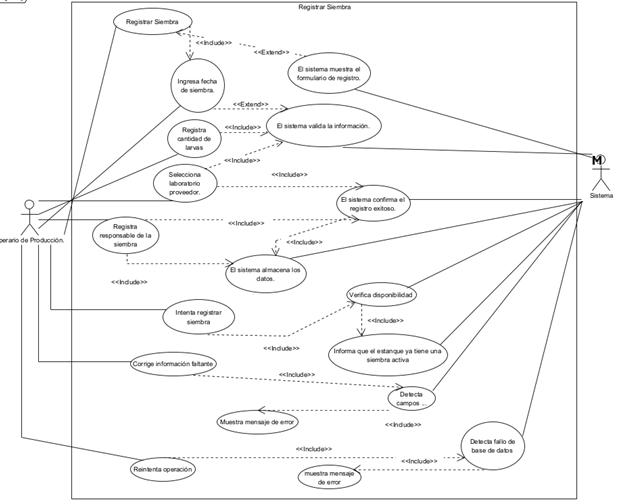
\includegraphics[width=0.75\textwidth]{Imagen1.png}
\caption{Diagrama del Caso de Uso CU-01: Registrar Siembra}
\end{figure}

\subsubsection{CU-02: Registrar Parámetros del Agua}

Especificación completa reproducida en el requisito RF-06 (Sección~3.1).

\begin{figure}[H]
\centering
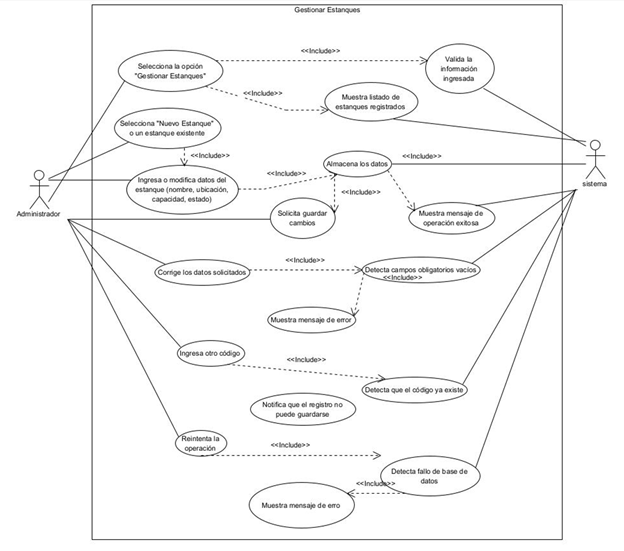
\includegraphics[width=0.75\textwidth]{Imagen2.png}
\caption{Diagrama del Caso de Uso CU-02: Registrar Parámetros del Agua}
\end{figure}

\subsubsection{CU-03: Generar Reporte Productivo}

Especificación completa reproducida en el requisito RF-16 (Sección~3.1).

\begin{figure}[H]
\centering
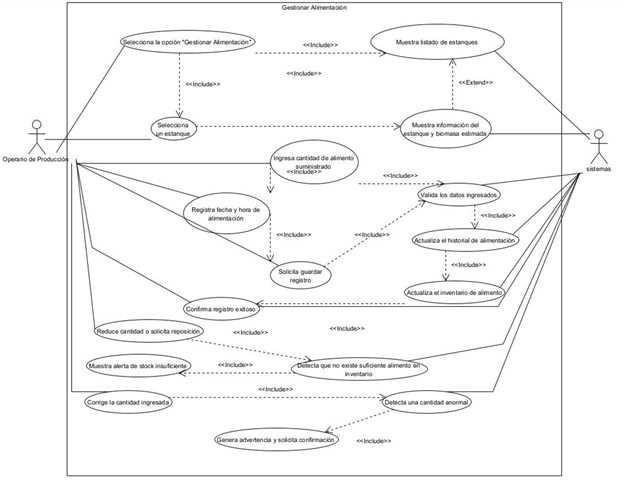
\includegraphics[width=0.75\textwidth]{Imagen3.png}
\caption{Diagrama del Caso de Uso CU-03: Generar Reporte Productivo}
\end{figure}

\subsubsection{CU-04 a CU-08}

Para los siguientes cinco casos de uso, el documento original únicamente
proporciona el diagrama UML correspondiente, sin especificación textual de
flujo principal, flujos alternativos ni excepciones. Dicha especificación
textual detallada queda, por tanto, \textbf{pendiente de definir en futuras
iteraciones}; su descripción funcional general se documenta en los
requisitos RF-01/RF-02 (CU-04), RF-12/RF-13 (CU-05), RF-15 (CU-06), RF-17/RF-18
(CU-07) y RF-10 (CU-08).

\begin{figure}[H]\centering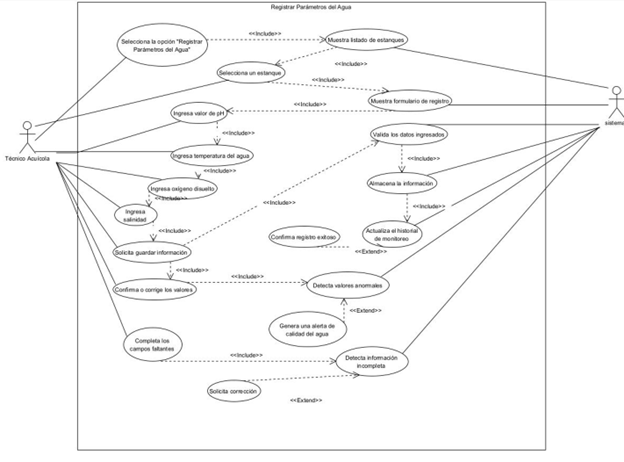
\includegraphics[width=0.75\textwidth]{Imagen4.png}\caption{Diagrama del Caso de Uso CU-04: Gestionar Estanques}\end{figure}
\begin{figure}[H]\centering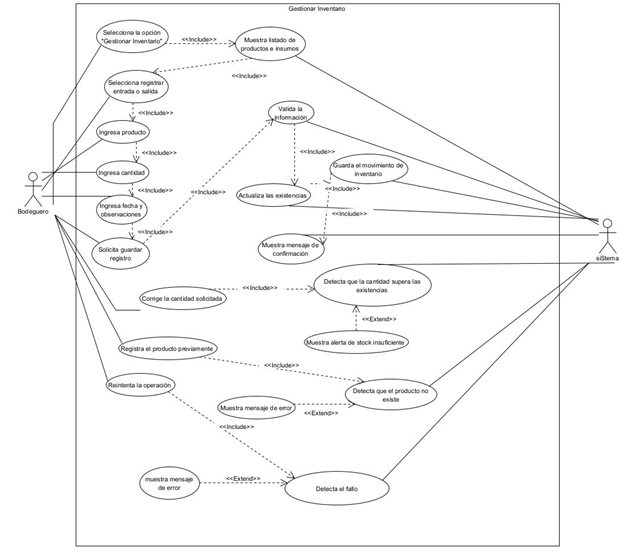
\includegraphics[width=0.75\textwidth]{Imagen5.png}\caption{Diagrama del Caso de Uso CU-05: Gestionar Inventario}\end{figure}
\begin{figure}[H]\centering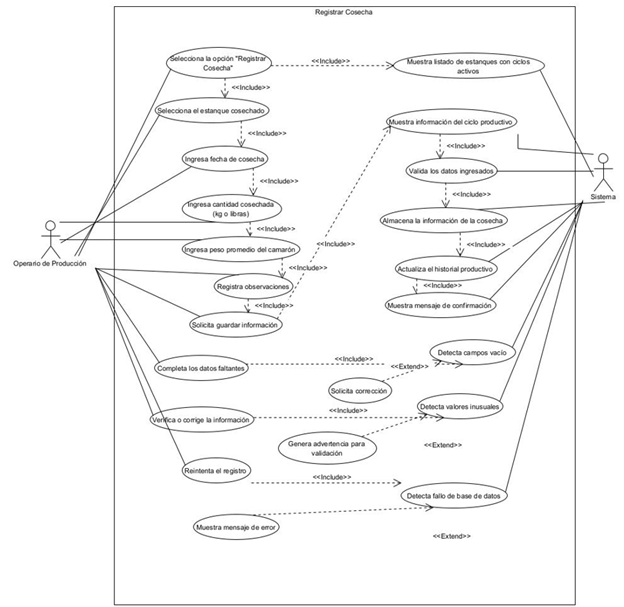
\includegraphics[width=0.75\textwidth]{Imagen6.png}\caption{Diagrama del Caso de Uso CU-06: Registrar Cosecha}\end{figure}
\begin{figure}[H]\centering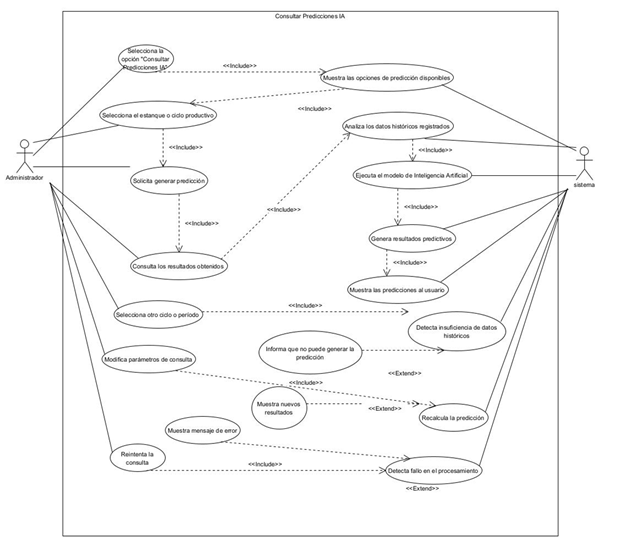
\includegraphics[width=0.75\textwidth]{Imagen7.png}\caption{Diagrama del Caso de Uso CU-07: Consultar Predicciones IA}\end{figure}
\begin{figure}[H]\centering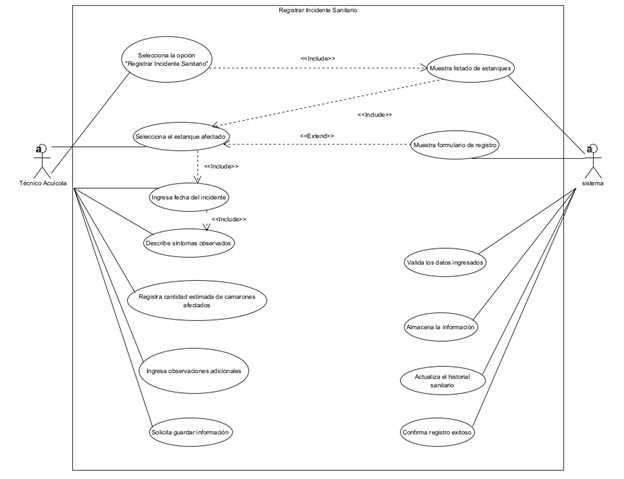
\includegraphics[width=0.75\textwidth]{Imagen8.png}\caption{Diagrama del Caso de Uso CU-08: Registrar Incidentes Sanitarios}\end{figure}

\subsection{Modelo de metas i*~2.0}

El marco i*~2.0 modela el entorno socio-técnico del sistema como una red de
actores con intenciones (metas, tareas, recursos y vulnerabilidades) y
dependencias entre ellos, produciendo dos modelos complementarios: el
\textit{Strategic Dependency Model} (SD), que representa las dependencias
entre actores, y el \textit{Strategic Rationale Model} (SR), que descompone
las intenciones internas del actor principal \cite{Yu1995,Kavakli2002}.

\subsubsection{Dependencias estratégicas más críticas (modelo SD)}

\begin{longtable}{|p{2.6cm}|p{4.0cm}|p{2.0cm}|p{5.2cm}|}
\caption{Dependencias estratégicas críticas --- modelo SD} \\
\hline
\textbf{Depender} & \textbf{Dependum} & \textbf{Dependee} & \textbf{Riesgo asociado} \\
\hline
\endfirsthead
\hline
\textbf{Depender} & \textbf{Dependum} & \textbf{Dependee} & \textbf{Riesgo asociado} \\
\hline
\endhead
Técnico Acuícola & Inmediatez y precisión de las alertas & AquaGest &
En modo offline, la alerta local puede no llegar al supervisor (conflicto
RF-06/RNF-01, resuelto mediante negociación, Sección~9.5) \\
\hline
Operario de Campo & Disponibilidad offline del sistema & AquaGest &
Sin acceso offline, el operario registra en papel, comprometiendo la
integridad de los datos \\
\hline
AquaGest & Continuidad del inventario crítico & Proveedor de Insumos &
Si el proveedor no responde, el sistema alerta (RF-12) pero no puede
garantizar la reposición \\
\hline
\end{longtable}

\subsubsection{Metas principales del actor Sistema AquaGest (modelo SR)}

\begin{longtable}{|p{1.3cm}|p{11.3cm}|}
\caption{Metas principales especificadas en el modelo i*~2.0} \\
\hline
\textbf{ID} & \textbf{Enunciado (condición del mundo) y requisitos que la satisfacen} \\
\hline
\endfirsthead
\hline
\textbf{ID} & \textbf{Enunciado (condición del mundo) y requisitos que la satisfacen} \\
\hline
\endhead
M1 & Centralización de datos operativos: todos los datos operativos de los
ciclos productivos de Biofina están almacenados de forma centralizada,
consistente y recuperable. Requisitos que la satisfacen: RF-01 a RF-15,
RNF-01, RNF-04. \\
\hline
M2 & Apoyo oportuno a la toma de decisiones: los usuarios con rol de gestión
disponen de información analítica actual (alertas, reportes y predicciones)
en el momento en que la necesitan. Requisitos que la satisfacen: RF-05, RF-06,
RF-07, RF-09, RF-10, RF-16. \\
\hline
M3 & Integridad y seguridad de la información: la información es accesible
únicamente por usuarios autorizados según su rol y se conserva íntegra ante
fallos de conectividad o energía. Requisitos que la satisfacen: RNF-01,
RNF-02, RNF-04, REST-03. \\
\hline
M4 & Reducción de pérdidas por decisiones tardías: las pérdidas productivas
atribuibles a intervenciones tardías se reducen en al menos un 20\,\% respecto
al semestre anterior a la implantación. Requisitos que la satisfacen: RF-05,
RF-06, RF-10, RF-12, RF-17. \\
\hline
\end{longtable}

El análisis interpretativo del modelo i*~2.0 confirma que la meta M2 concentra
el mayor número de contribuciones positivas del sistema, mientras que la única
contribución negativa (\textit{hurt}) identificada corresponde a la tarea de
predicción de cosecha por IA (RF-17), lo que refuerza su clasificación como
requisito \textit{Could} en MoSCoW y \textit{Atractivo} en Kano hasta contar
con volumen suficiente de datos históricos \cite{Pohl2010,Yu1995}.


% ============================================================
\section{Reglas de Negocio}
% ============================================================

Las siguientes reglas de negocio fueron identificadas a partir del análisis de
la entrevista de elicitación, los casos de uso y el proceso de negociación de
requisitos documentados en el proyecto original \cite{Pohl2010,ISO29148:2018}.

\begin{longtable}{|p{1.6cm}|p{11.4cm}|}
\caption{Reglas de negocio del sistema AquaGest} \\
\hline
\textbf{ID} & \textbf{Regla de negocio} \\
\hline
\endfirsthead
\hline
\textbf{ID} & \textbf{Regla de negocio} \\
\hline
\endhead
RN-01 & Un estanque no puede tener más de una siembra activa simultáneamente;
si ya existe un ciclo productivo en curso, el sistema debe impedir el registro
de una nueva siembra (flujo alternativo FA2 de RF-03). \\ \hline
RN-02 & Toda siembra que exceda la capacidad máxima de larvas calculada para
un estanque (RF-02) constituye una sobrecarga y debe registrarse
obligatoriamente junto con su justificación. \\ \hline
RN-03 & Toda medición de un parámetro del agua fuera del rango óptimo
configurado debe generar una alerta local inmediata en el dispositivo del
técnico responsable, independientemente de la disponibilidad de conexión a
internet (RF-06, según la resolución del conflicto RF-06/RNF-01 documentada en
el Acta de Negociación, Sección~9.5). \\ \hline
RN-04 & En modo offline, las alertas generadas deben almacenarse localmente y
sincronizarse como notificaciones \textit{push} diferidas al administrador o
supervisor en un plazo máximo de 5 minutos tras restablecerse la conexión
(Acta de Negociación, Sección~9.5). \\ \hline
RN-05 & Toda mortalidad registrada por encima del umbral configurado debe
generar una alerta automática dirigida al técnico acuícola responsable
(RF-10). \\ \hline
RN-06 & El stock de un insumo que caiga por debajo del nivel mínimo configurado
debe generar automáticamente una alerta de reposición visible para el
administrador (RF-12). \\ \hline
RN-07 & El módulo de predicción de cosecha por inteligencia artificial (RF-17)
solo puede ejecutarse cuando existan al menos tres ciclos productivos
históricos con grameos semanales completos; en caso contrario, el sistema debe
rechazar la ejecución e informar la insuficiencia de datos. \\ \hline
RN-08 & El acceso a cada funcionalidad y punto de acceso del sistema debe
restringirse según el rol asignado al usuario autenticado (administrador,
técnico u operario), rechazando las solicitudes fuera de rol con código de
respuesta HTTP 403 (RNF-SEG-03, Sección~3.2). \\ \hline
RN-09 & Una cuenta de usuario debe bloquearse temporalmente durante 15 minutos
después de tres intentos fallidos consecutivos de autenticación, notificando
al administrador del evento (RNF-SEG-01). \\ \hline
RN-10 & Ante un fallo del sensor IoT de monitoreo del agua, el sistema debe
permitir el ingreso manual de los valores, registrando explícitamente la
fuente del dato como ``manual'' para fines de trazabilidad (excepción E1 de
RF-06). \\ \hline
\end{longtable}

No se identificó, en el documento original, ninguna otra regla de negocio
adicional más allá de las aquí enumeradas; cualquier regla no listada se
considera \textbf{pendiente de definir en futuras iteraciones}.

% ============================================================
\section{Requisitos de Calidad}
% ============================================================

Los requisitos de calidad del sistema AquaGest se organizan conforme a las
características del modelo de calidad de producto de la norma
ISO/IEC 25010:2023 \cite{ISO25010:2023}, integrando los requisitos no
funcionales especificados en la Sección~3.2 y los requisitos de seguridad
derivados del análisis del \textit{misuse scenario} MS-01.

\begin{longtable}{|p{3.4cm}|p{9.6cm}|}
\caption{Requisitos de calidad organizados por atributo (ISO/IEC 25010:2023)} \\
\hline
\textbf{Atributo de calidad} & \textbf{Requisitos asociados} \\
\hline
\endfirsthead
\hline
\textbf{Atributo de calidad} & \textbf{Requisitos asociados} \\
\hline
\endhead
Adecuación funcional & RF-01 a RF-18 (Sección~3.1), verificados contra el
conjunto de necesidades declaradas por los interesados durante la entrevista y
el cuestionario \cite{ISO25010:2023}. \\ \hline
Eficiencia de desempeño & RNF-03: tiempo de respuesta inferior a 3 segundos
con hasta 15 usuarios concurrentes. \\ \hline
Compatibilidad & REST-01: compatibilidad con los navegadores Chrome y
Firefox, sin instalación en dispositivos de campo. \\ \hline
Capacidad de interacción (usabilidad) & \textit{Softgoal} de usabilidad en
condiciones de campo identificado en el modelo i*~2.0 (Sección~4.3) para el
Operario de Campo; sin métrica cuantitativa definida. \textbf{Pendiente de
definir en futuras iteraciones.} \\ \hline
Fiabilidad & RNF-01 (disponibilidad $\geq$ 99\,\% y modo offline) y RNF-04
(persistencia de transacciones sin pérdida ante fallos). \\ \hline
Seguridad & RNF-02 (autenticación multifactor y RBAC), RNF-SEG-01 (bloqueo
tras intentos fallidos), RNF-SEG-02 (hash seguro de contraseñas) y RNF-SEG-03
(control de acceso por rol a nivel de endpoint), derivados del análisis del
\textit{misuse scenario} MS-01 (Sección~6.1). \\ \hline
Mantenibilidad & \textit{Softgoal} de mantenibilidad del código identificado en
el modelo SR del actor Sistema AquaGest (Sección~4.3); sin métrica
cuantitativa definida. \textbf{Pendiente de definir en futuras iteraciones.} \\ \hline
Flexibilidad (portabilidad) & Sin información específica en el documento
original. \textbf{Pendiente de definir en futuras iteraciones.} \\ \hline
\end{longtable}

\subsection{Misuse Scenario: Acceso No Autorizado al Sistema (MS-01)}

El \textit{misuse scenario} permite identificar requisitos de seguridad desde
la perspectiva del atacante, siguiendo el enfoque de ingeniería de requisitos
orientada a la seguridad \cite{Pohl2010,SWEBOK2024}.

\begin{table}[H]
\centering
\caption{Misuse Scenario MS-01: Acceso No Autorizado al Sistema AquaGest}
\begin{tabular}{|p{3.8cm}|p{10.4cm}|}
\hline
\textbf{Campo} & \textbf{Descripción} \\
\hline
Actor malicioso & Usuario externo sin credenciales válidas (atacante) \\ \hline
Objetivo del atacante & Obtener acceso no autorizado a información
confidencial sobre producción, inventario y cosechas de Biofina; modificar
registros para encubrir pérdidas o alterar datos de inventario \\ \hline
Escenario de ataque & (1) El atacante localiza la URL del sistema AquaGest.
(2) Prueba combinaciones de usuario y contraseña (fuerza bruta/diccionario).
(3) Obtiene acceso mediante credenciales comprometidas o débiles.
(4) Consulta datos sensibles de producción, costos e inventario.
(5) Modifica registros de producción o inventario. \\ \hline
Riesgos identificados & Pérdida de confidencialidad de datos productivos y
financieros; manipulación de registros; daños económicos por decisiones
basadas en datos adulterados \\ \hline
Requisitos de seguridad derivados & RNF-SEG-01, RNF-SEG-02 y RNF-SEG-03
(Sección~3.2) \\ \hline
\end{tabular}
\end{table}

% ============================================================
\section{Trazabilidad}
% ============================================================

La matriz de trazabilidad relaciona las necesidades del cliente --- expresadas
como hallazgos y acuerdos de la entrevista de elicitación (Sección~9.2) --- con
los requisitos funcionales y no funcionales que las satisfacen, conforme al
principio de trazabilidad establecido por la norma ISO/IEC/IEEE 29148:2018
\cite{ISO29148:2018,Pohl2010}.

\begin{longtable}{|p{4.6cm}|p{3.6cm}|p{3.4cm}|p{2.0cm}|}
\caption{Matriz de trazabilidad: necesidad del cliente $\rightarrow$ RF $\rightarrow$ RNF} \\
\hline
\textbf{Necesidad del cliente} & \textbf{Requisito funcional} & \textbf{Requisito no funcional} & \textbf{Meta i*} \\
\hline
\endfirsthead
\hline
\textbf{Necesidad del cliente} & \textbf{Requisito funcional} & \textbf{Requisito no funcional} & \textbf{Meta i*} \\
\hline
\endhead
Centralizar el registro de estanques, hoy gestionado manualmente & RF-01, RF-02 & RNF-04 & M1 \\ \hline
Trazar el ciclo productivo desde la siembra & RF-03, RF-04 & RNF-04 & M1 \\ \hline
Automatizar la alerta de crecimiento inferior al esperado & RF-05 & --- & M2, M4 \\ \hline
Generar alertas automáticas ante parámetros del agua fuera de rango & RF-06, RF-07 & RNF-01 & M2, M4 \\ \hline
Automatizar el cálculo de ración de alimento y su eficiencia (FCR) & RF-08, RF-09 & --- & M1, M2 \\ \hline
Formalizar el historial sanitario y alertar mortalidad anormal & RF-10 & --- & M2, M4 \\ \hline
Gestionar empleados y asignación de tareas & RF-11 & RNF-02 & M1 \\ \hline
Evitar faltantes críticos de insumos (balanceado, medicinas) & RF-12, RF-13 & --- & M4 \\ \hline
Reducir el reporte verbal de fallas de equipos y planificar mantenimiento & RF-14 & --- & M1 \\ \hline
Registrar cosechas y controlar el costo de producción & RF-15 & --- & M1 \\ \hline
Reducir el tiempo de elaboración manual de reportes gerenciales & RF-16 & RNF-03 & M2 \\ \hline
Anticipar el momento óptimo de cosecha con base en datos históricos & RF-17 & --- & M2, M4 \\ \hline
Detectar tempranamente anomalías en la calidad del agua & RF-18 & --- & M2, M4 \\ \hline
Operar en zonas de conectividad limitada sin perder información & --- & RNF-01, RNF-04 & M1, M3 \\ \hline
Proteger la información productiva y financiera frente a accesos no
autorizados & --- & RNF-02, RNF-SEG-01, RNF-SEG-02, RNF-SEG-03 & M3 \\ \hline
Cumplir con la normativa ecuatoriana de protección de datos & --- & REST-03 & M3 \\ \hline
No disponer de dispositivos administrados en campo & --- & REST-01 & --- \\ \hline
No interrumpir los procesos operativos actuales durante la implantación & --- & REST-02 & --- \\ \hline
\end{longtable}

Esta matriz relaciona directamente los hallazgos de la entrevista y del
cuestionario digital (Sección~9.2 y 9.3) con los requisitos consolidados en la
Sección~3, y con las metas del modelo i*~2.0 documentadas en la Sección~4.3, lo
que permite verificar que ningún requisito carece de una necesidad de origen
que lo justifique \cite{ISO29148:2018}.

% ============================================================
\section{Riesgos}
% ============================================================

Se documentan los riesgos identificados durante la planificación de la
elicitación y los riesgos estratégicos derivados del análisis del modelo
i*~2.0, conforme al dominio de incertidumbre del PMBoK 7.\textsuperscript{a}
edición \cite{PMI2021,Robertson2012}.

\subsection{Riesgos de la elicitación}

\begin{longtable}{|p{4.4cm}|p{6.0cm}|p{2.8cm}|}
\caption{Riesgos identificados durante la elicitación de requisitos} \\
\hline
\textbf{Riesgo} & \textbf{Descripción} & \textbf{Probabilidad / Impacto} \\
\hline
\endfirsthead
\hline
\textbf{Riesgo} & \textbf{Descripción} & \textbf{Probabilidad / Impacto} \\
\hline
\endhead
Indisponibilidad del administrador & El interesado principal puede tener
compromisos operativos imprevistos que impidan o interrumpan la sesión de
elicitación. & Media / Alta \\ \hline
Conocimiento tácito no articulado & El administrador puede omitir procesos que
considera obvios, produciendo un inventario de requisitos incompleto
\cite{Pohl2010}. & Alta / Alta \\ \hline
Baja tasa de respuesta al cuestionario & El personal operativo puede no
responder el cuestionario en el plazo establecido, reduciendo la
representatividad de los resultados. & Media / Media \\ \hline
Ambigüedad terminológica & Interesados de distintas áreas pueden usar términos
diferentes para el mismo concepto del dominio \cite{IREB2023}. & Alta / Media \\ \hline
Sesgo de deseabilidad social & Los participantes del cuestionario pueden
responder según lo que creen que el equipo espera oír \cite{Pacheco2018}. & Media / Media \\ \hline
Conflictos entre perspectiva gerencial y operativa & Las respuestas del
administrador pueden diferir de las del personal operativo, generando
requisitos contradictorios que requieren negociación \cite{Pohl2010,Robertson2012}. & Media / Alta \\ \hline
\end{longtable}

\subsection{Riesgos estratégicos derivados del modelo i*~2.0}

\begin{enumerate}[nosep]
  \item \textbf{Riesgo residual en la entrega de alertas offline.} Aun con la
  solución de alerta local más sincronización diferida (RF-06, RN-03, RN-04),
  el supervisor no recibe la alerta en tiempo real mientras el técnico
  permanece en campo sin conexión; este riesgo residual debe documentarse y
  monitorearse en iteraciones posteriores \cite{Yu1995}.
  \item \textbf{Riesgo de abandono del sistema por baja usabilidad de campo.}
  Si la interfaz offline no resulta suficientemente simple e intuitiva para el
  Operario de Campo, existe el riesgo de que el registro vuelva a realizarse en
  papel, comprometiendo la integridad del inventario y de los reportes
  directivos \cite{ISO25010:2023}.
  \item \textbf{Riesgo de dependencia no controlable del proveedor de
  insumos.} Las alertas de stock mínimo (RF-12) son efectivas solo si el
  proveedor de insumos responde oportunamente; una falla en la cadena de
  suministro no puede ser resuelta por el sistema, únicamente notificada
  \cite{Yu1995}.
  \item \textbf{Riesgo de pérdida de confianza por predicciones de IA poco
  precisas.} Si el módulo de predicción de cosecha (RF-17) genera resultados
  poco confiables por insuficiencia de datos históricos en las primeras
  iteraciones, puede erosionar la confianza del administrador en el sistema en
  su conjunto; de allí su clasificación como \textit{Could} en MoSCoW.
  \item \textbf{Riesgo de seguridad por acceso no autorizado.} Documentado en
  el \textit{misuse scenario} MS-01 (Sección~6.1): pérdida de confidencialidad
  y manipulación de registros productivos y financieros ante un ataque de
  fuerza bruta o credenciales débiles, mitigado mediante RNF-SEG-01 a
  RNF-SEG-03.
\end{enumerate}


% ============================================================
\section{Anexos}
% ============================================================

\subsection{Guía de entrevista semiestructurada}

La entrevista se realizó el 28 de mayo de 2026 con el señor Christian Leonel
Franco Anchundia, administrador de Biofina (camaronera ubicada en El Guasmo),
utilizando una guía organizada en nueve bloques temáticos correspondientes a
los dominios funcionales del sistema AquaGest, siguiendo la recomendación de
estructurar la entrevista evitando saltos temáticos que dificulten el
seguimiento del interesado \cite{Pohl2010,IREB2023}.

\begin{longtable}{|p{3.6cm}|p{9.4cm}|}
\caption{Bloques temáticos de la guía de entrevista} \\
\hline
\textbf{Bloque} & \textbf{Temas cubiertos} \\
\hline
\endfirsthead
\hline
\textbf{Bloque} & \textbf{Temas cubiertos} \\
\hline
\endhead
1. Información General & Nombre, cargo y responsabilidades del entrevistado. \\ \hline
2. Gestión de Estanques & Registro actual de estanques, determinación de capacidad de siembra, sobrecarga y seguimiento de estado. \\ \hline
3. Control de Siembras & Información registrada por siembra, seguimiento del desarrollo, indicadores y tipos de alerta. \\ \hline
4. Monitoreo de Parámetros del Agua & Parámetros monitoreados, frecuencia, responsables y acciones ante valores fuera de rango. \\ \hline
5. Gestión de Alimentación & Cálculo de ración, factores de ajuste, registro de consumo y evaluación de eficiencia. \\ \hline
6. Gestión de Empleados & Información de registro, tipos de roles y control de tareas. \\ \hline
7. Historial Sanitario & Detección de enfermedades, procedimientos y registro de información. \\ \hline
8. Gestión de Cosechas & Información registrada, cálculo de rendimiento, comparación entre ciclos y costos. \\ \hline
9. Reportes y Análisis & Tipos de reportes utilizados, decisiones basadas en ellos y necesidades de alertas automáticas. \\ \hline
\end{longtable}

\subsection{Acta de entrevista de elicitación}

\begin{table}[H]
\centering
\caption{Resumen del acta de entrevista de elicitación}
\begin{tabular}{|p{4cm}|p{9cm}|}
\hline
\textbf{Elemento} & \textbf{Detalle} \\
\hline
Proyecto & Sistema de Gestión Inteligente de Camaronera (AquaGest) \\ \hline
Fecha & 28 de mayo de 2026 \\ \hline
Modalidad & Videollamada \\ \hline
Duración & 45 minutos aproximadamente \\ \hline
Stakeholder entrevistado & Christian Leonel Franco Anchundia, Administrador de
Biofina --- Camaronera El Guasmo \\ \hline
Equipo entrevistador & Ariel Omar Castro Bajaña e integrantes del grupo de
Ingeniería de Software (UTEQ) \\ \hline
Objetivo & Identificar necesidades operativas y requisitos funcionales para el
sistema AquaGest \\ \hline
Principales acuerdos & Validar los requisitos mediante cuestionario digital,
priorizar el monitoreo de agua, implementar alertas automáticas, generar
reportes automáticos y analizar funcionalidades basadas en inteligencia
artificial \\ \hline
Resultados obtenidos & Se identificaron requisitos relacionados con gestión de
estanques, siembras, monitoreo de agua, alimentación, historial sanitario,
cosechas, reportes e inteligencia artificial \\ \hline
\end{tabular}
\end{table}

\textbf{Hallazgos identificados:} los estanques se gestionaban de forma manual
sin sistema centralizado; el seguimiento de crecimiento mediante grameos
semanales carecía de alertas automáticas; el registro de parámetros del agua
era manual; el cálculo del FCR no se realizaba sistemáticamente; los
incidentes sanitarios carecían de historial formal con evidencia fotográfica;
los reportes se generaban manualmente, retrasando la toma de decisiones
gerenciales.

\begin{figure}[H]
\centering
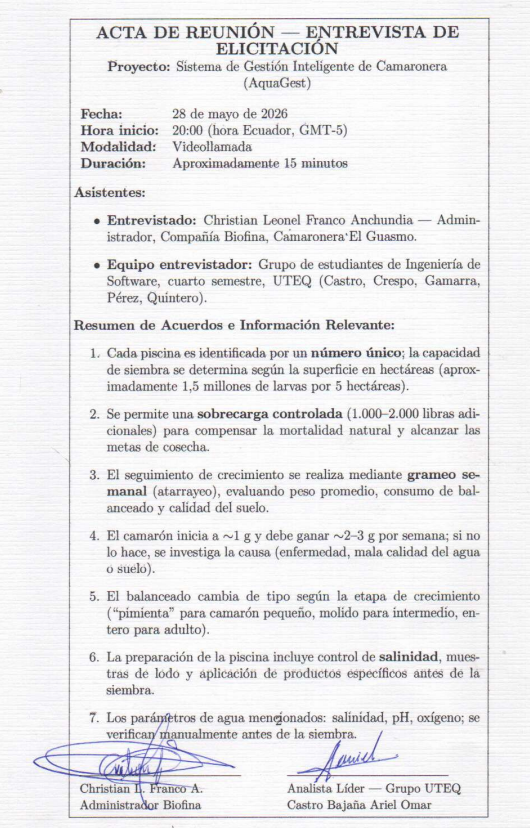
\includegraphics[width=0.6\textwidth]{actaentrevista.png}
\caption{Acta de entrevista de elicitación realizada al administrador de
Biofina para la identificación de requisitos del sistema AquaGest.}
\end{figure}

\begin{figure}[H]
\centering
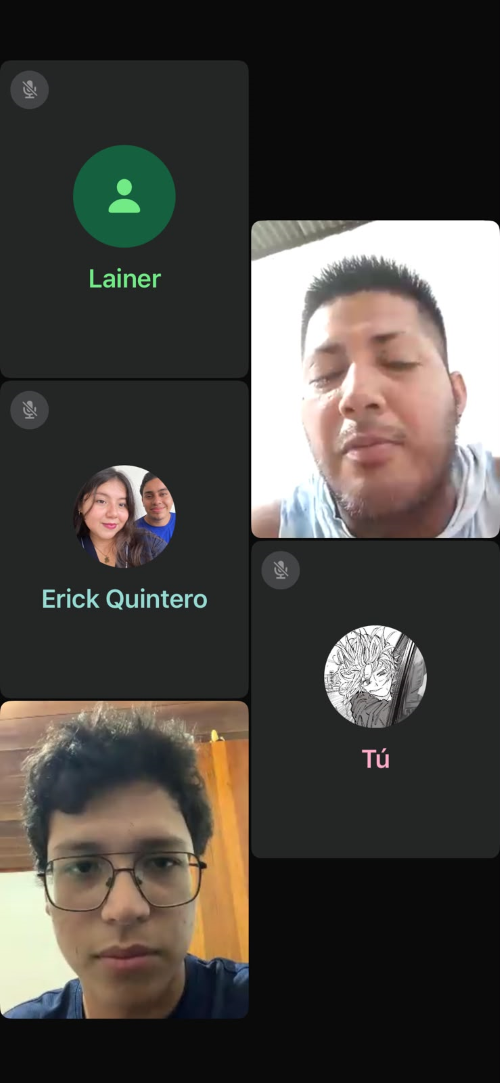
\includegraphics[width=0.5\textwidth]{entrevistafoto.png}
\caption{Evidencia fotográfica de la entrevista semiestructurada realizada al
stakeholder principal.}
\end{figure}

\subsection{Cuestionario digital}

El cuestionario digital, implementado mediante Google Forms y distribuido a
las ocho áreas operativas de Biofina, fue respondido por doce participantes
pertenecientes a siete de dichas áreas: producción (25\,\%), mantenimiento
(17\,\%), cosecha (17\,\%), alimentación (17\,\%), calidad del agua (8\,\%),
logística/bodega (8\,\%) y calidad/empacadora (8\,\%)
\cite{Robertson2012,IREB2023}. Entre las tendencias identificadas destacan: el
100\,\% de los participantes de producción emplea métodos manuales de
seguimiento del crecimiento; el 100\,\% de los participantes reporta monitoreo
del agua varias veces al día; el 67\,\% determina la ración de alimento por
biomasa estimada; el 83\,\% de cosecha determina el momento óptimo por peso
promedio; y la demora en reportes fue identificada como el principal problema
administrativo. La sección de escala Likert del instrumento no registró
respuestas válidas de ningún participante, limitación que se documenta
explícitamente conforme al principio de no generar análisis inexistente
\cite{ISO29148:2018}.

\subsection{Sesión de brainstorming}

La sesión de brainstorming, realizada el 30 de mayo de 2026 con una duración
de 20 minutos, generó quince ideas mediante el protocolo estándar de
generación libre y diferimiento del juicio \cite{Pohl2010}. De estas ideas se
derivaron cinco nuevos requisitos crudos (RC-26 a RC-30) no cubiertos por la
entrevista ni el cuestionario: modo offline (RF-01/RNF-01), detección de
anomalías por aprendizaje automático (RF-18), control de acceso por roles
(RNF-02), registro de proveedores (RF-13) y gráficas de evolución histórica
(RF-16). Las ideas restantes --- dashboard en tiempo real, alerta por SMS,
recomendación automática de ración, registro fotográfico sanitario,
integración con balanzas digitales, control de turnos de empleados y mapa
visual de estanques --- no fueron promovidas a requisitos formales del
conjunto RC-01 a RC-30 y se documentan como \textbf{pendientes de definir en
futuras iteraciones} (véanse las Secciones 3.3 y 6).

\subsection{Acta de negociación de requisitos}

\begin{table}[H]
\centering
\caption{Acta de Negociación de Requisitos --- Sistema AquaGest}
\begin{tabular}{|p{4.0cm}|p{9.2cm}|}
\hline
\multicolumn{2}{|c|}{\textbf{ACTA DE NEGOCIACIÓN DE REQUISITOS --- Sistema AquaGest}} \\ \hline
Participantes & Christian Leonel Franco Anchundia (Administrador de Biofina);
Equipo de desarrollo AquaGest \\ \hline
Requisitos en discusión & RF-06 (Alertas de parámetros del agua) y RNF-01
(Modo offline y disponibilidad $\geq$ 99\,\%) \\ \hline
Posición del stakeholder & Las alertas deben ser inmediatas: los primeros
30 minutos tras un desequilibrio del agua son críticos \\ \hline
Posición del equipo de IR & La arquitectura offline-first es un requisito no
negociable de disponibilidad, dado el entorno de campo \\ \hline
Solución acordada & Alertas locales inmediatas en el dispositivo del técnico y
notificaciones \textit{push} diferidas al supervisor al recuperar la conexión,
con un tiempo máximo de sincronización de 5 minutos \\ \hline
\end{tabular}
\end{table}

% ============================================================
%  BIBLIOGRAFÍA
% ============================================================
\bibliographystyle{ieeetr}
\bibliography{referencias}

\end{document}
